\section{Esempio d'uso}
Qui di seguito verrà illustrato un caso d'uso del sistema per il quale sono riportati screenshot dal punto di vista di due utenti. L'utente \emph{Andrea} partecipa alla partita dal cellulare, per cui l'interfaccia mostrata sarà quella mobile, mentre l'utente \emph{Piero} accede al client attraverso un browser da un PC desktop.




\begin{figure}[H]
    \centering
    \begin{minipage}{0.25\textwidth}
        \centering
        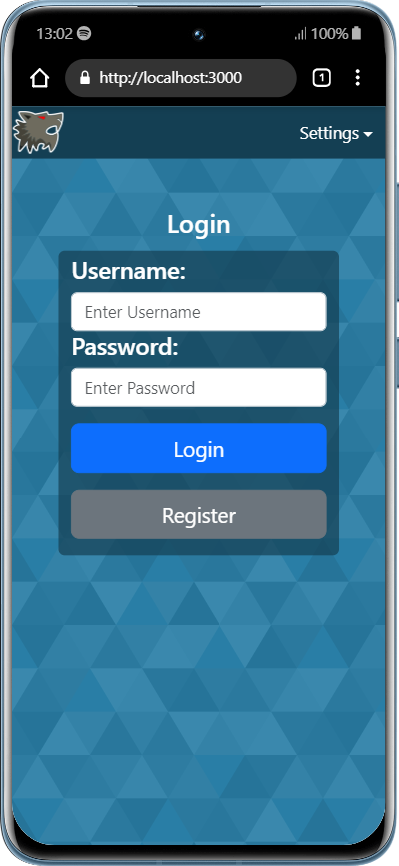
\includegraphics[width=0.95\textwidth]{img/screen/mobile/login_mobile.png}
    \end{minipage}\hfill
    \begin{minipage}{0.75\textwidth}
        \centering
        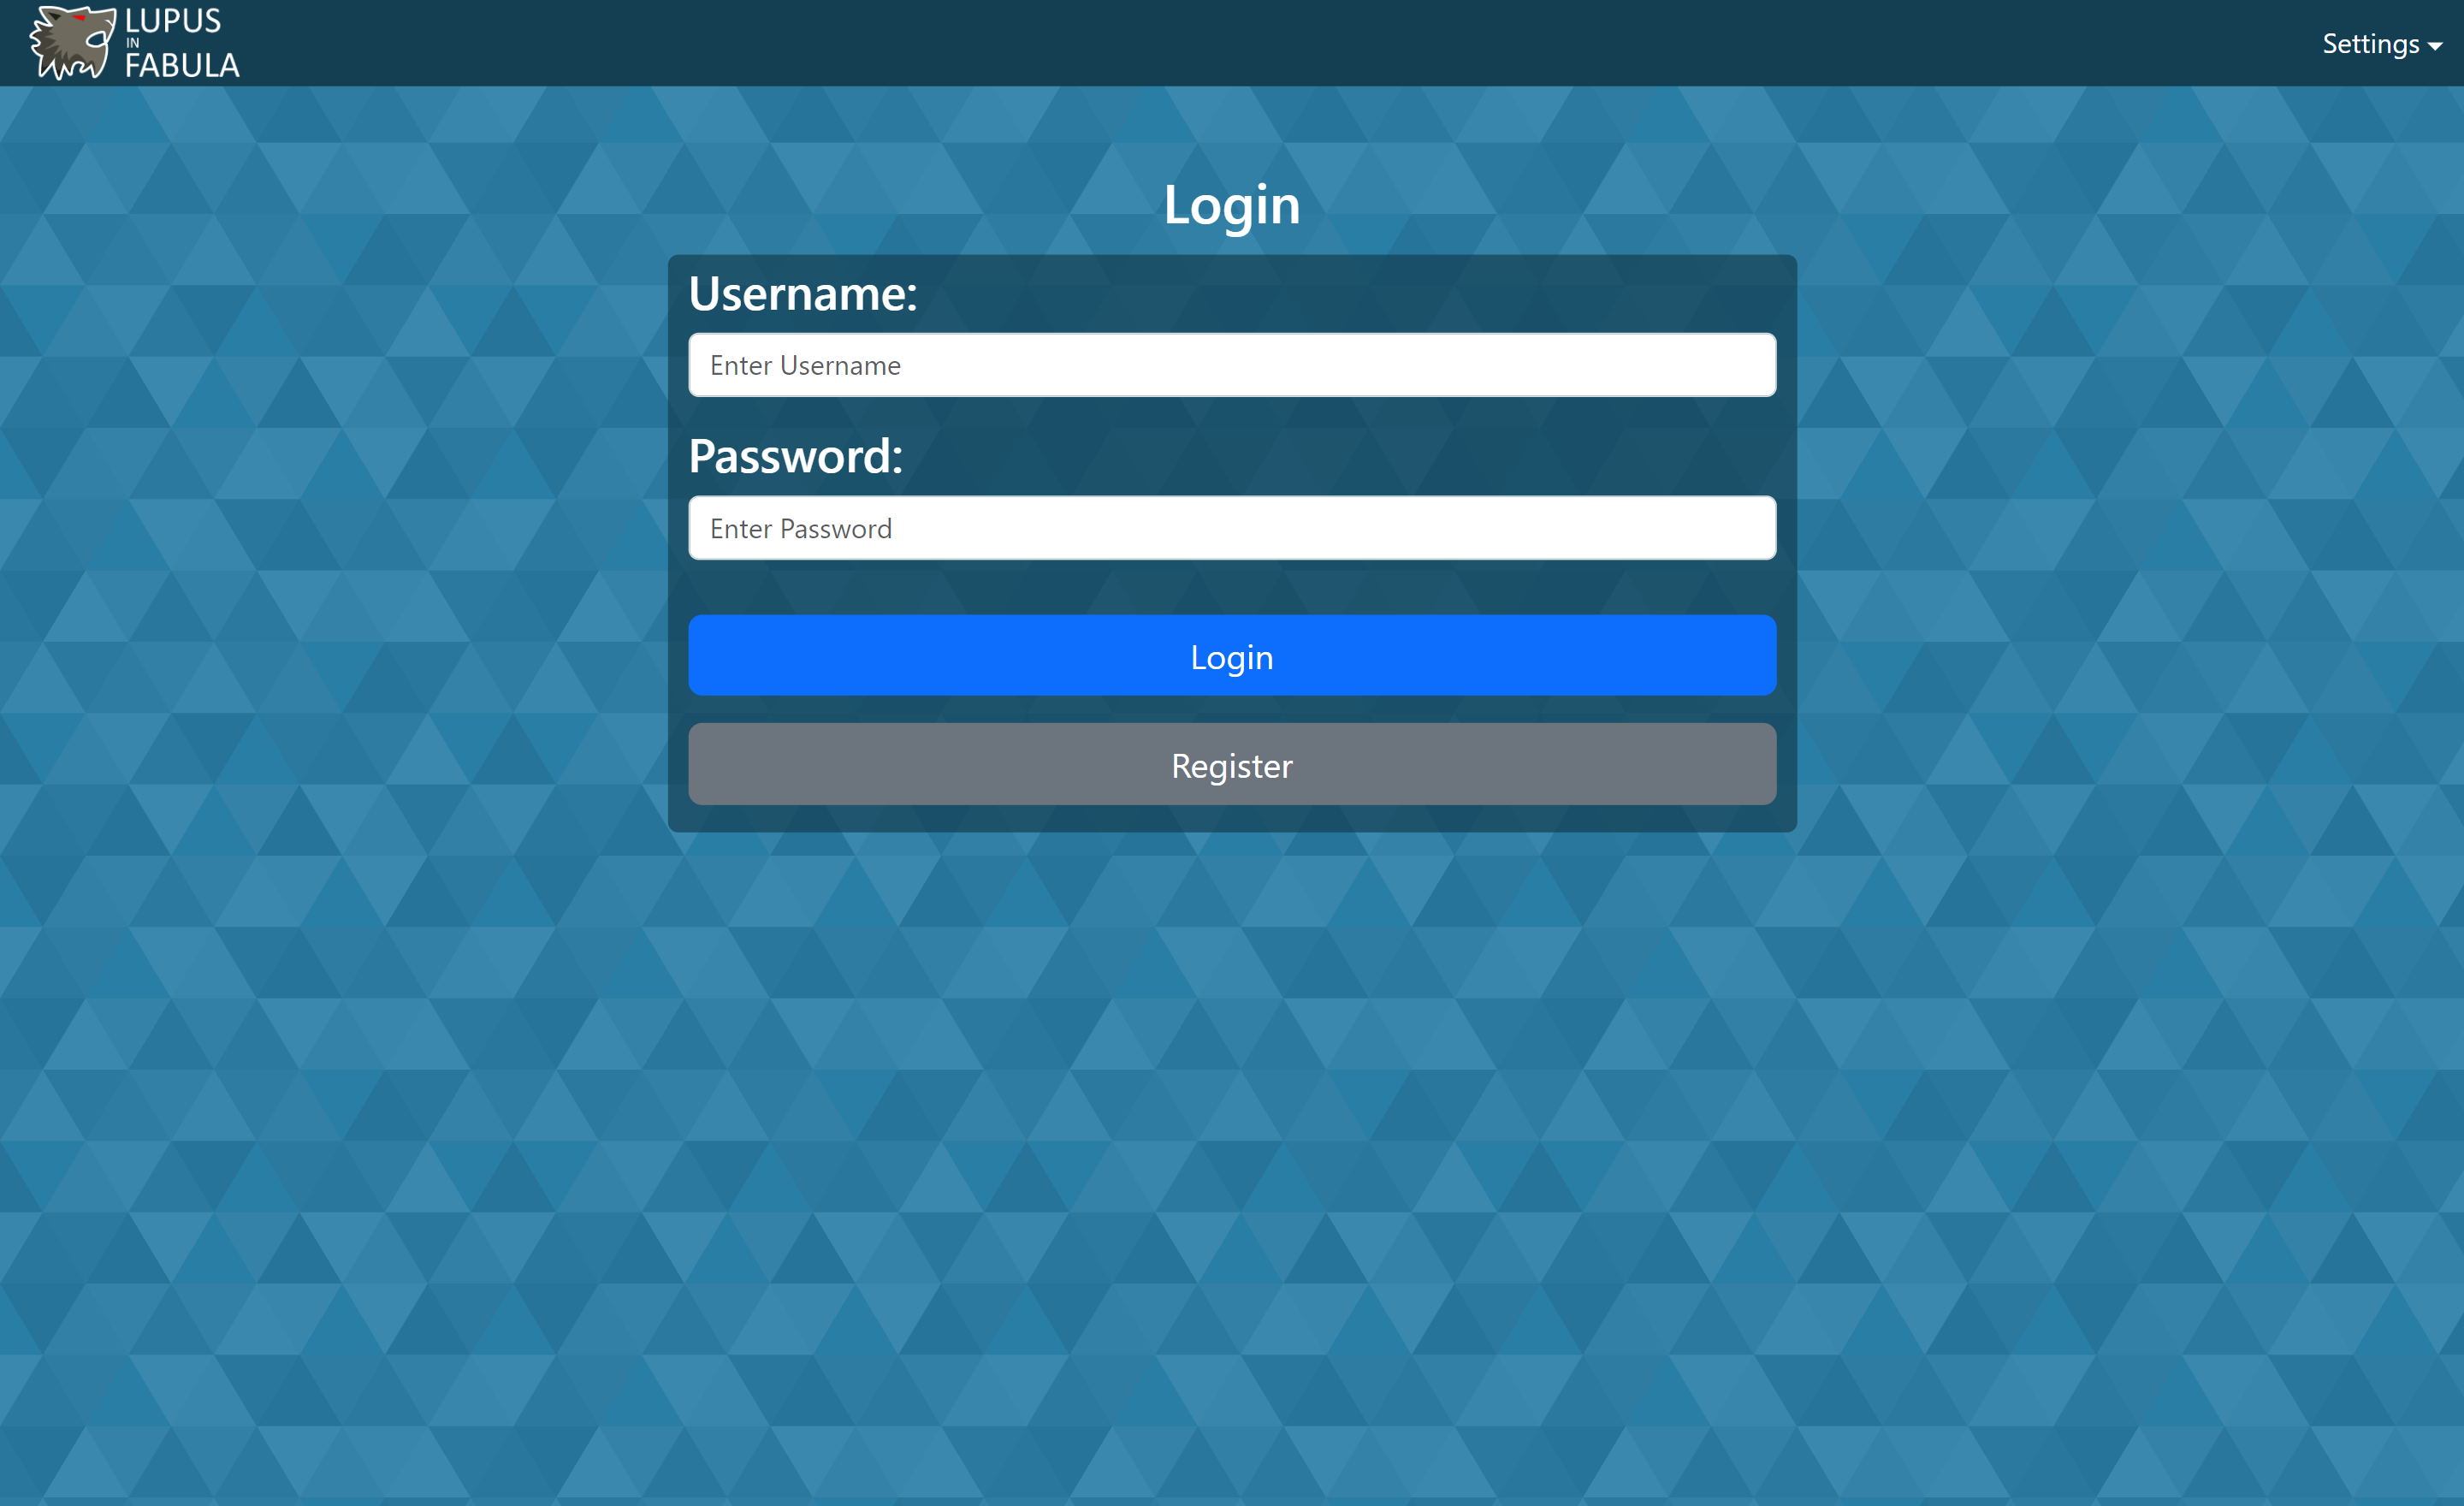
\includegraphics[width=0.95\textwidth]{img/screen/desktop/login_desktop.png}
    \end{minipage}
    \caption{Schermata di autenticazione}
    \label{fig:login_ui}
\end{figure}

Nella figura \ref{fig:login_ui} l'interfaccia proposta all'utente richiede l'inserimento delle credenziali per il login. Nel caso fosse la prima volta che si accede al servizio sarà necessario cliccare sul bottone \emph{Register} per registrarsi. Dal menù in alto a destra sarà possibile, come mostrato nella figura \ref{fig:language_ui}, selezionare la lingua nella quale utilizzare l'applicazione.


\begin{figure}[H]
    \centering
    \begin{minipage}{0.45\textwidth}
        \centering
        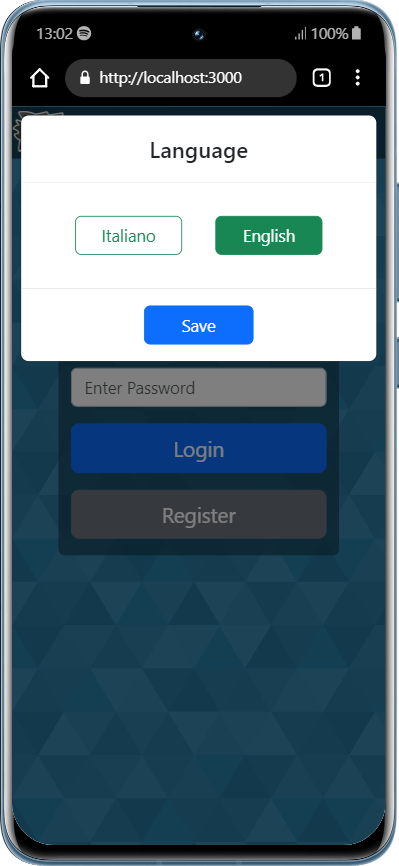
\includegraphics[width=0.8\textwidth]{img/screen/mobile/language_mobile.png}
    \end{minipage}
    \caption{Schermata di settaggio lingua}
    \label{fig:language_ui}
\end{figure}

Una volta effettuato l'accesso si avrà la possibilità nell'interfaccia \ref{fig:party_ui} di creare una stanza, o di unirsi a una già creata in precedenza, inserendo nell'apposito campo il codice univoco del \emph{party}.

\begin{figure}[H]
    \centering
    \begin{minipage}{0.25\textwidth}
        \centering
        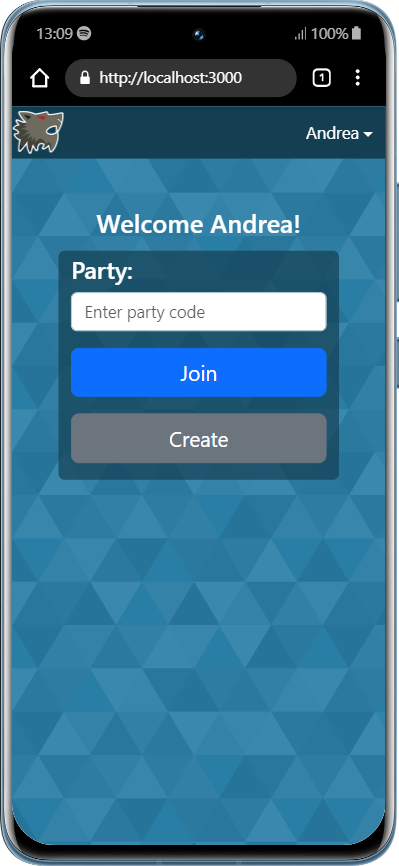
\includegraphics[width=0.95\textwidth]{img/screen/mobile/party_mobile.png}
    \end{minipage}\hfill
    \begin{minipage}{0.75\textwidth}
        \centering
        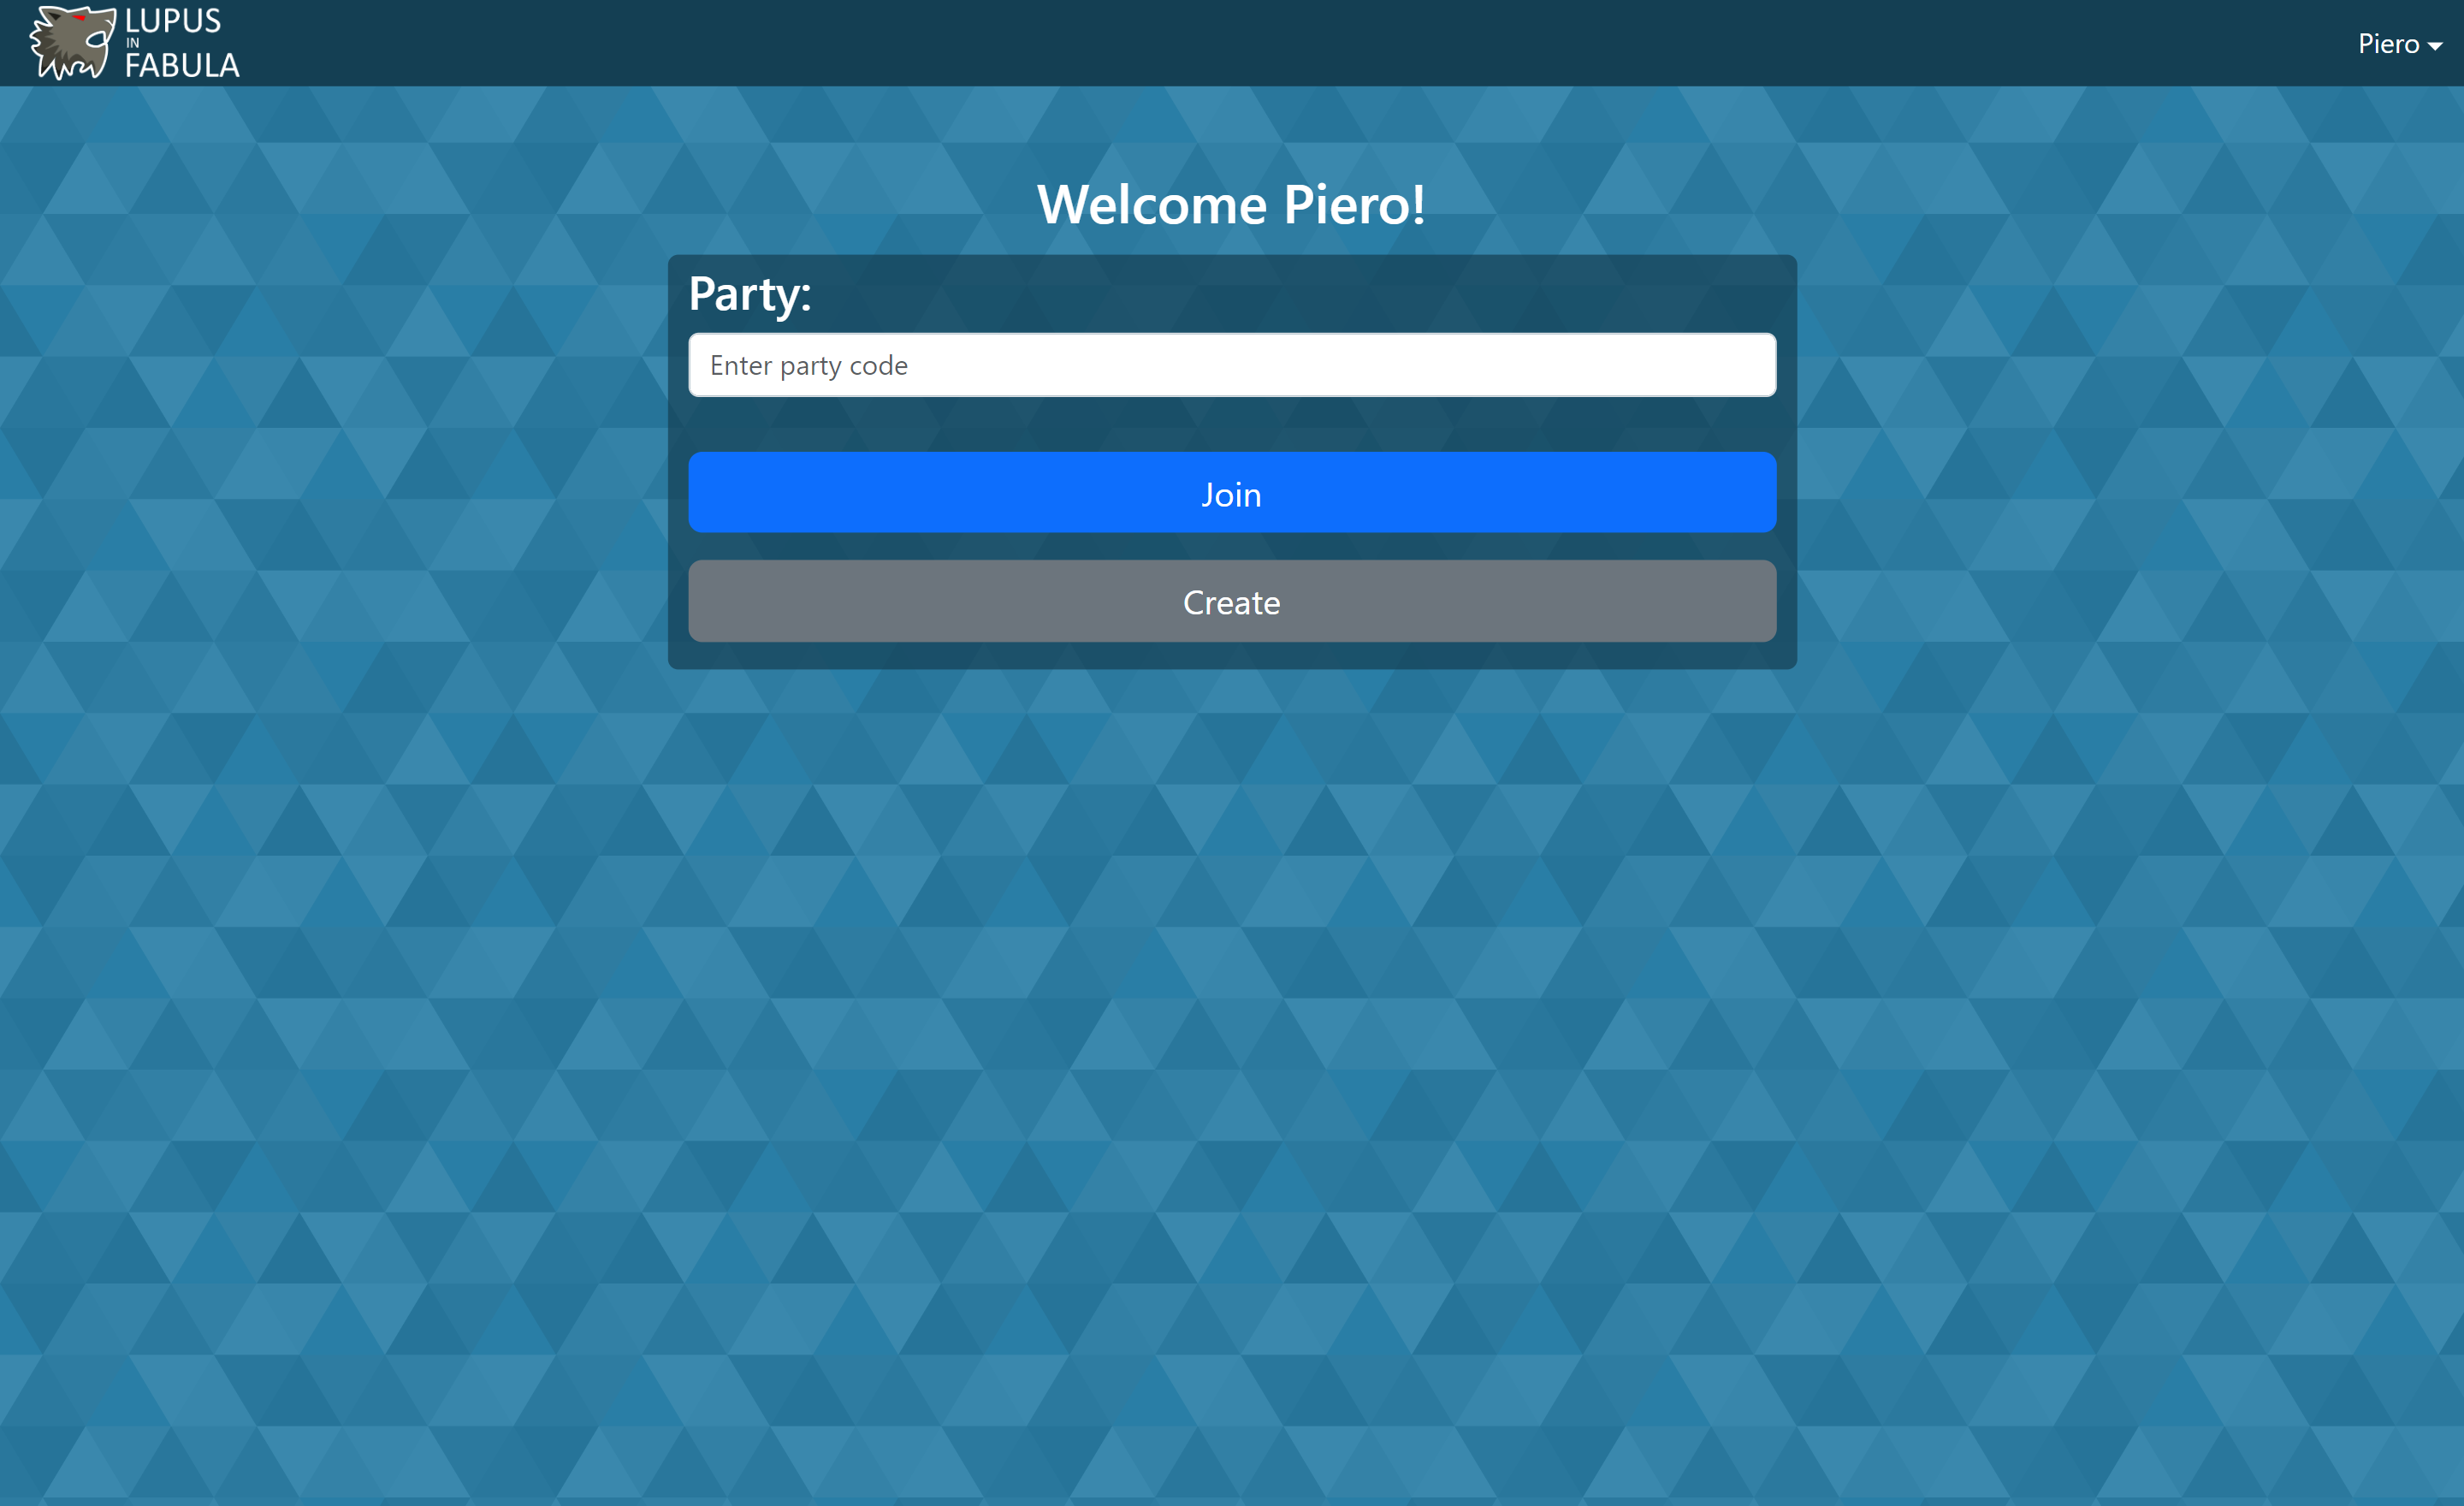
\includegraphics[width=0.95\textwidth]{img/screen/desktop/party_desktop.png}
    \end{minipage}
    \caption{Schermata di selezione party}
    \label{fig:party_ui}
\end{figure}

La schermata successiva che viene mostrata è una semplice \emph{lobby} all'interno della quale è possibile attendere tutti i partecipanti. I pulsanti nella parte bassa dello schermo danno la possibilità all'utente di lasciare la lobby e tornare alla schermata precedente, oppure di chiuderla proseguendo così a quella successiva.

\begin{figure}[H]
    \centering
    \begin{minipage}{0.25\textwidth}
        \centering
        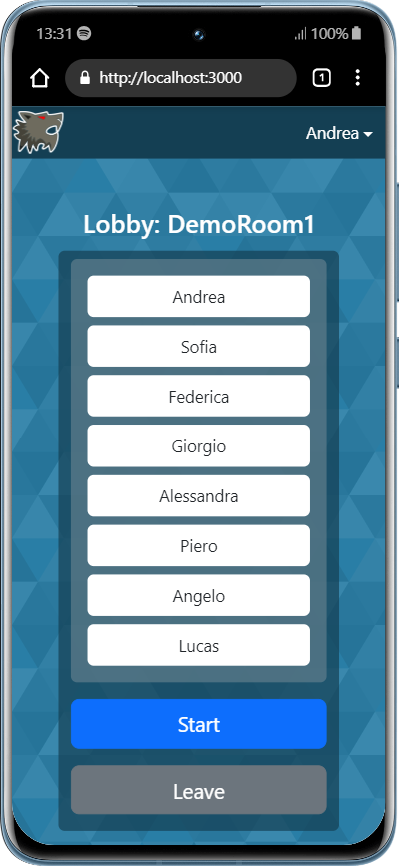
\includegraphics[width=0.95\textwidth]{img/screen/mobile/lobby_mobile.png}
    \end{minipage}\hfill
    \begin{minipage}{0.75\textwidth}
        \centering
        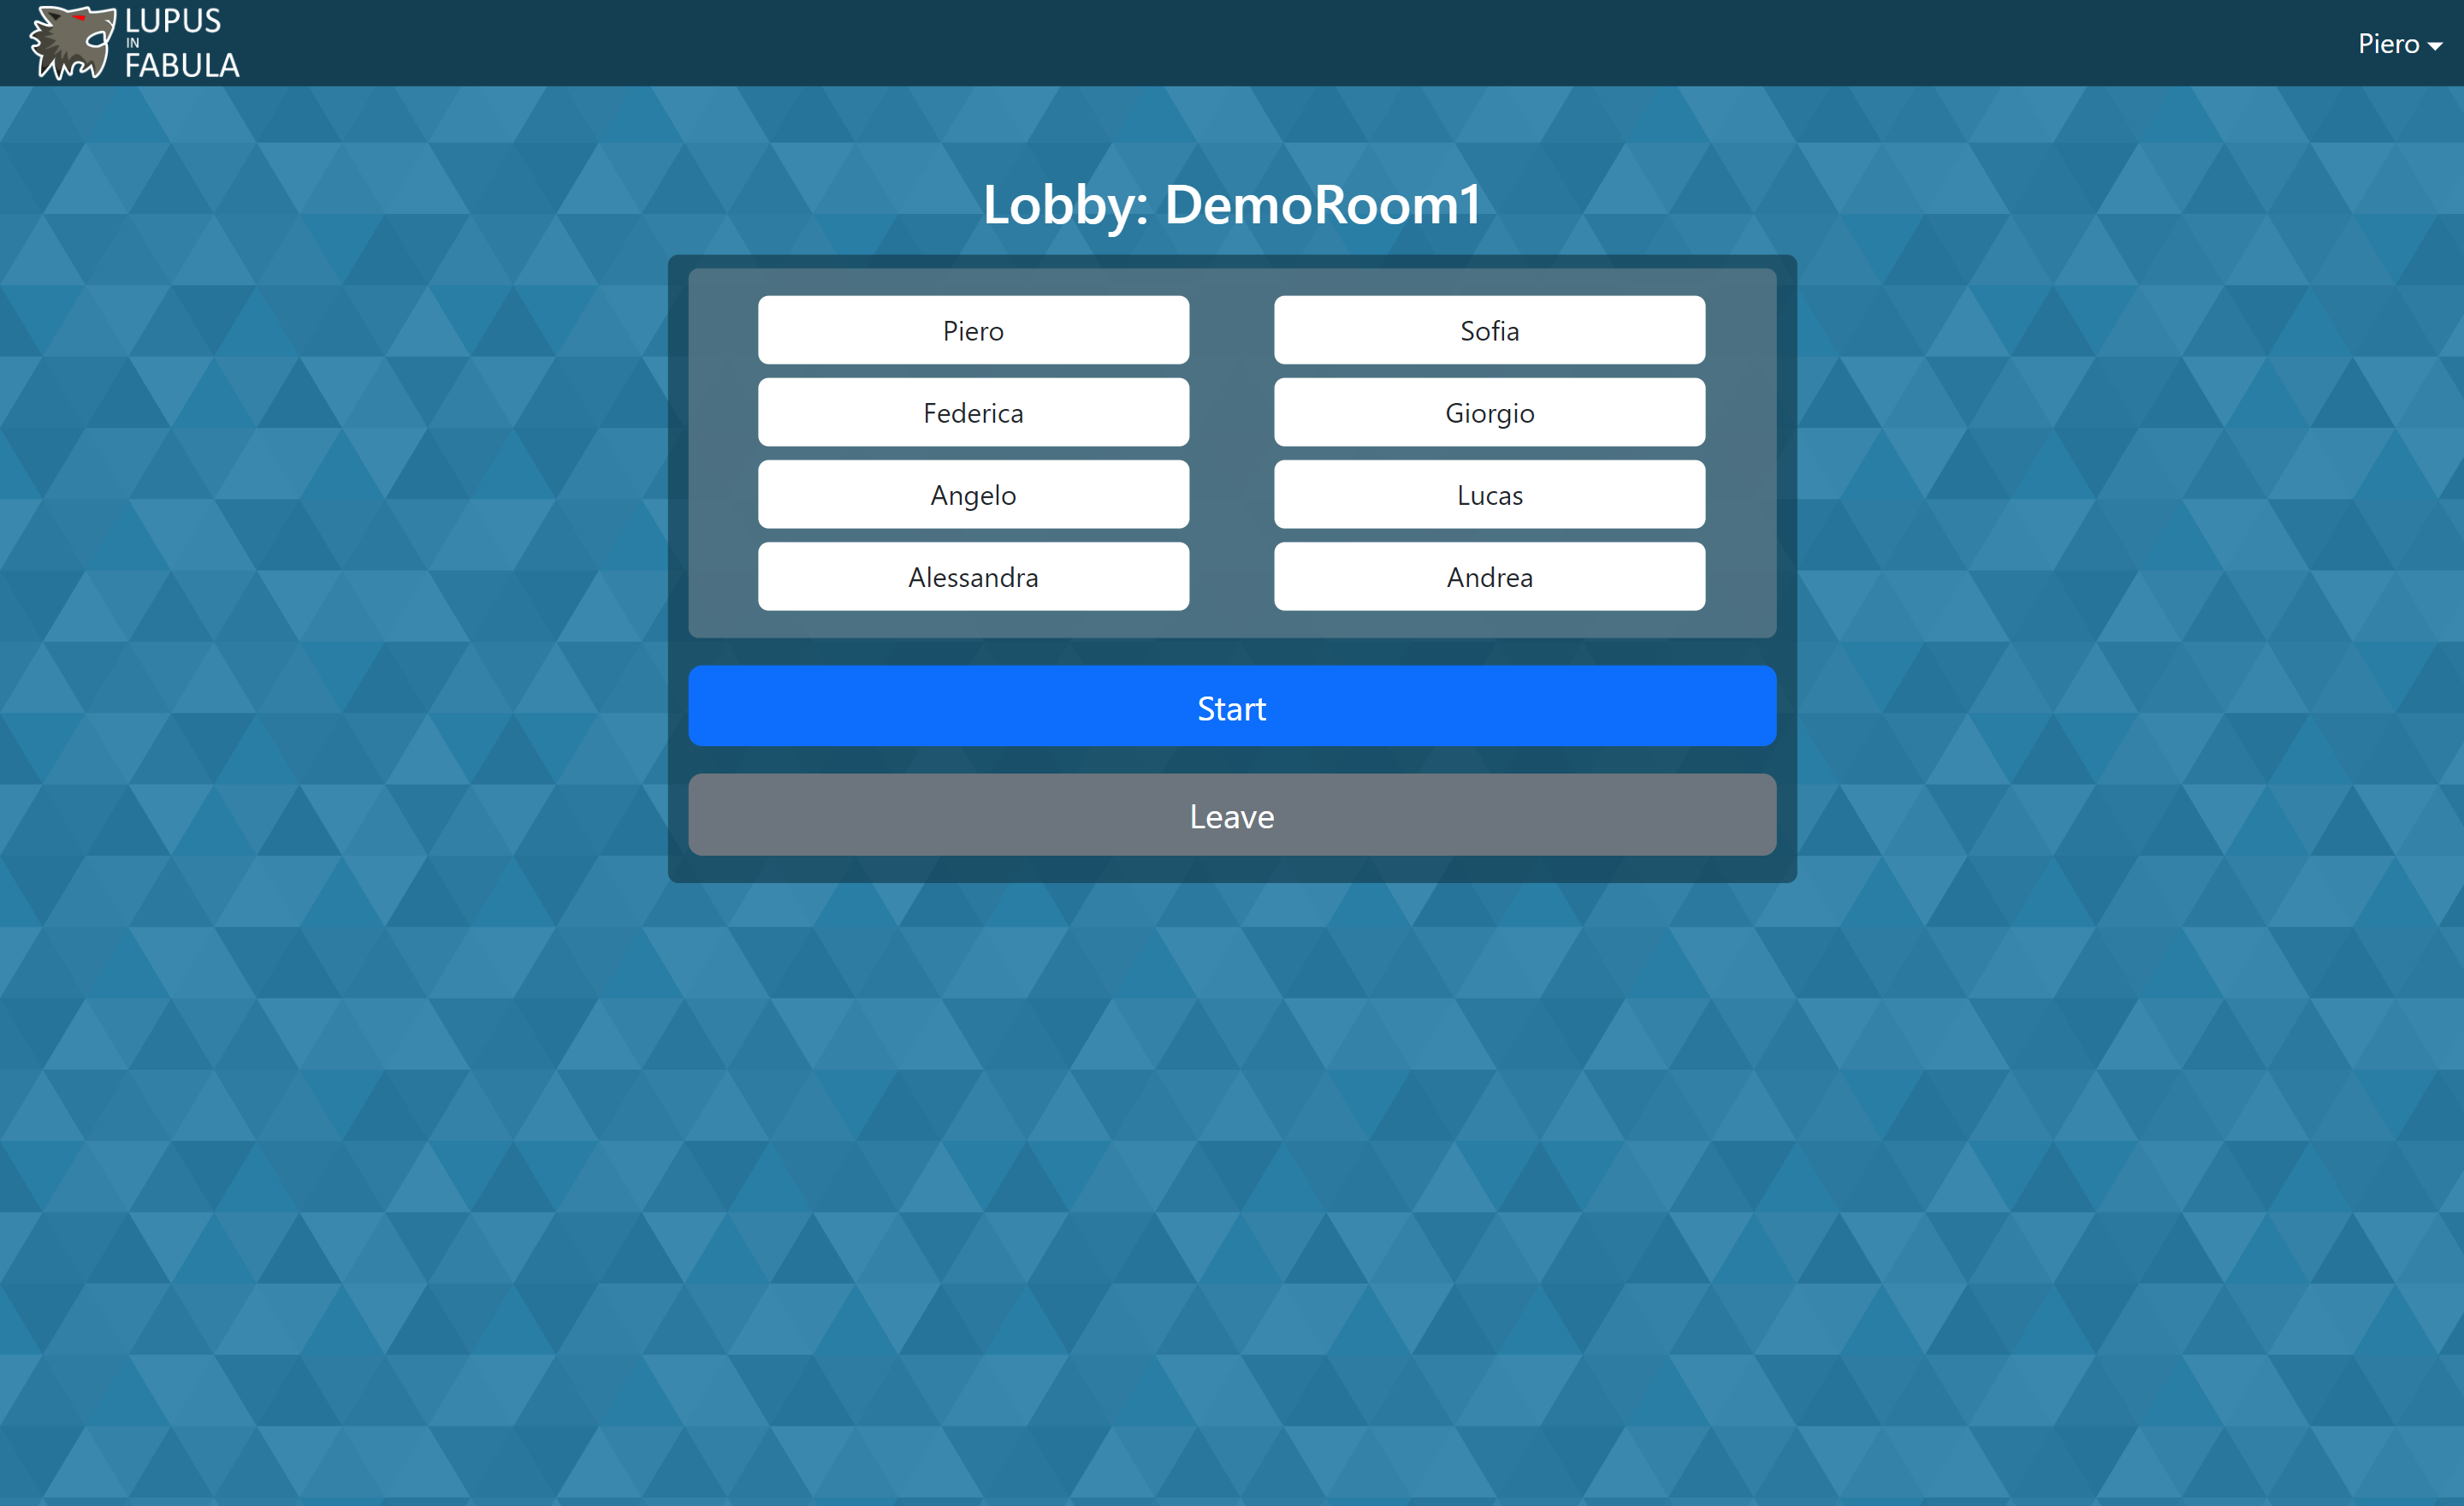
\includegraphics[width=0.95\textwidth]{img/screen/desktop/lobby_desktop.png}
    \end{minipage}
    \caption{Schermata di lobby}   
    \label{fig:lobby_ui}
\end{figure}

Dopo aver chiuso la lobby l'interfaccia mostrata aggiungerà la possibilità di modificare le impostazioni della partita prima di cominciare a giocare. La schermata di personalizzazione è mostrata nella figura \ref{fig:option_ui} e permette all'utente di modificare il numero di lupi presenti, oltre che di aggiungere o rimuovere i ruoli extra.


\begin{figure}[H]
    \centering
    \begin{minipage}{0.25\textwidth}
        \centering
        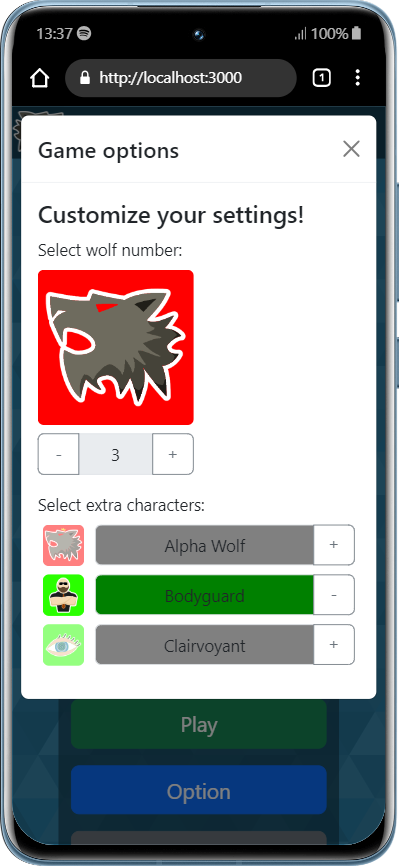
\includegraphics[width=0.95\textwidth]{img/screen/mobile/option_mobile.png}
    \end{minipage}\hfill
    \begin{minipage}{0.75\textwidth}
        \centering
        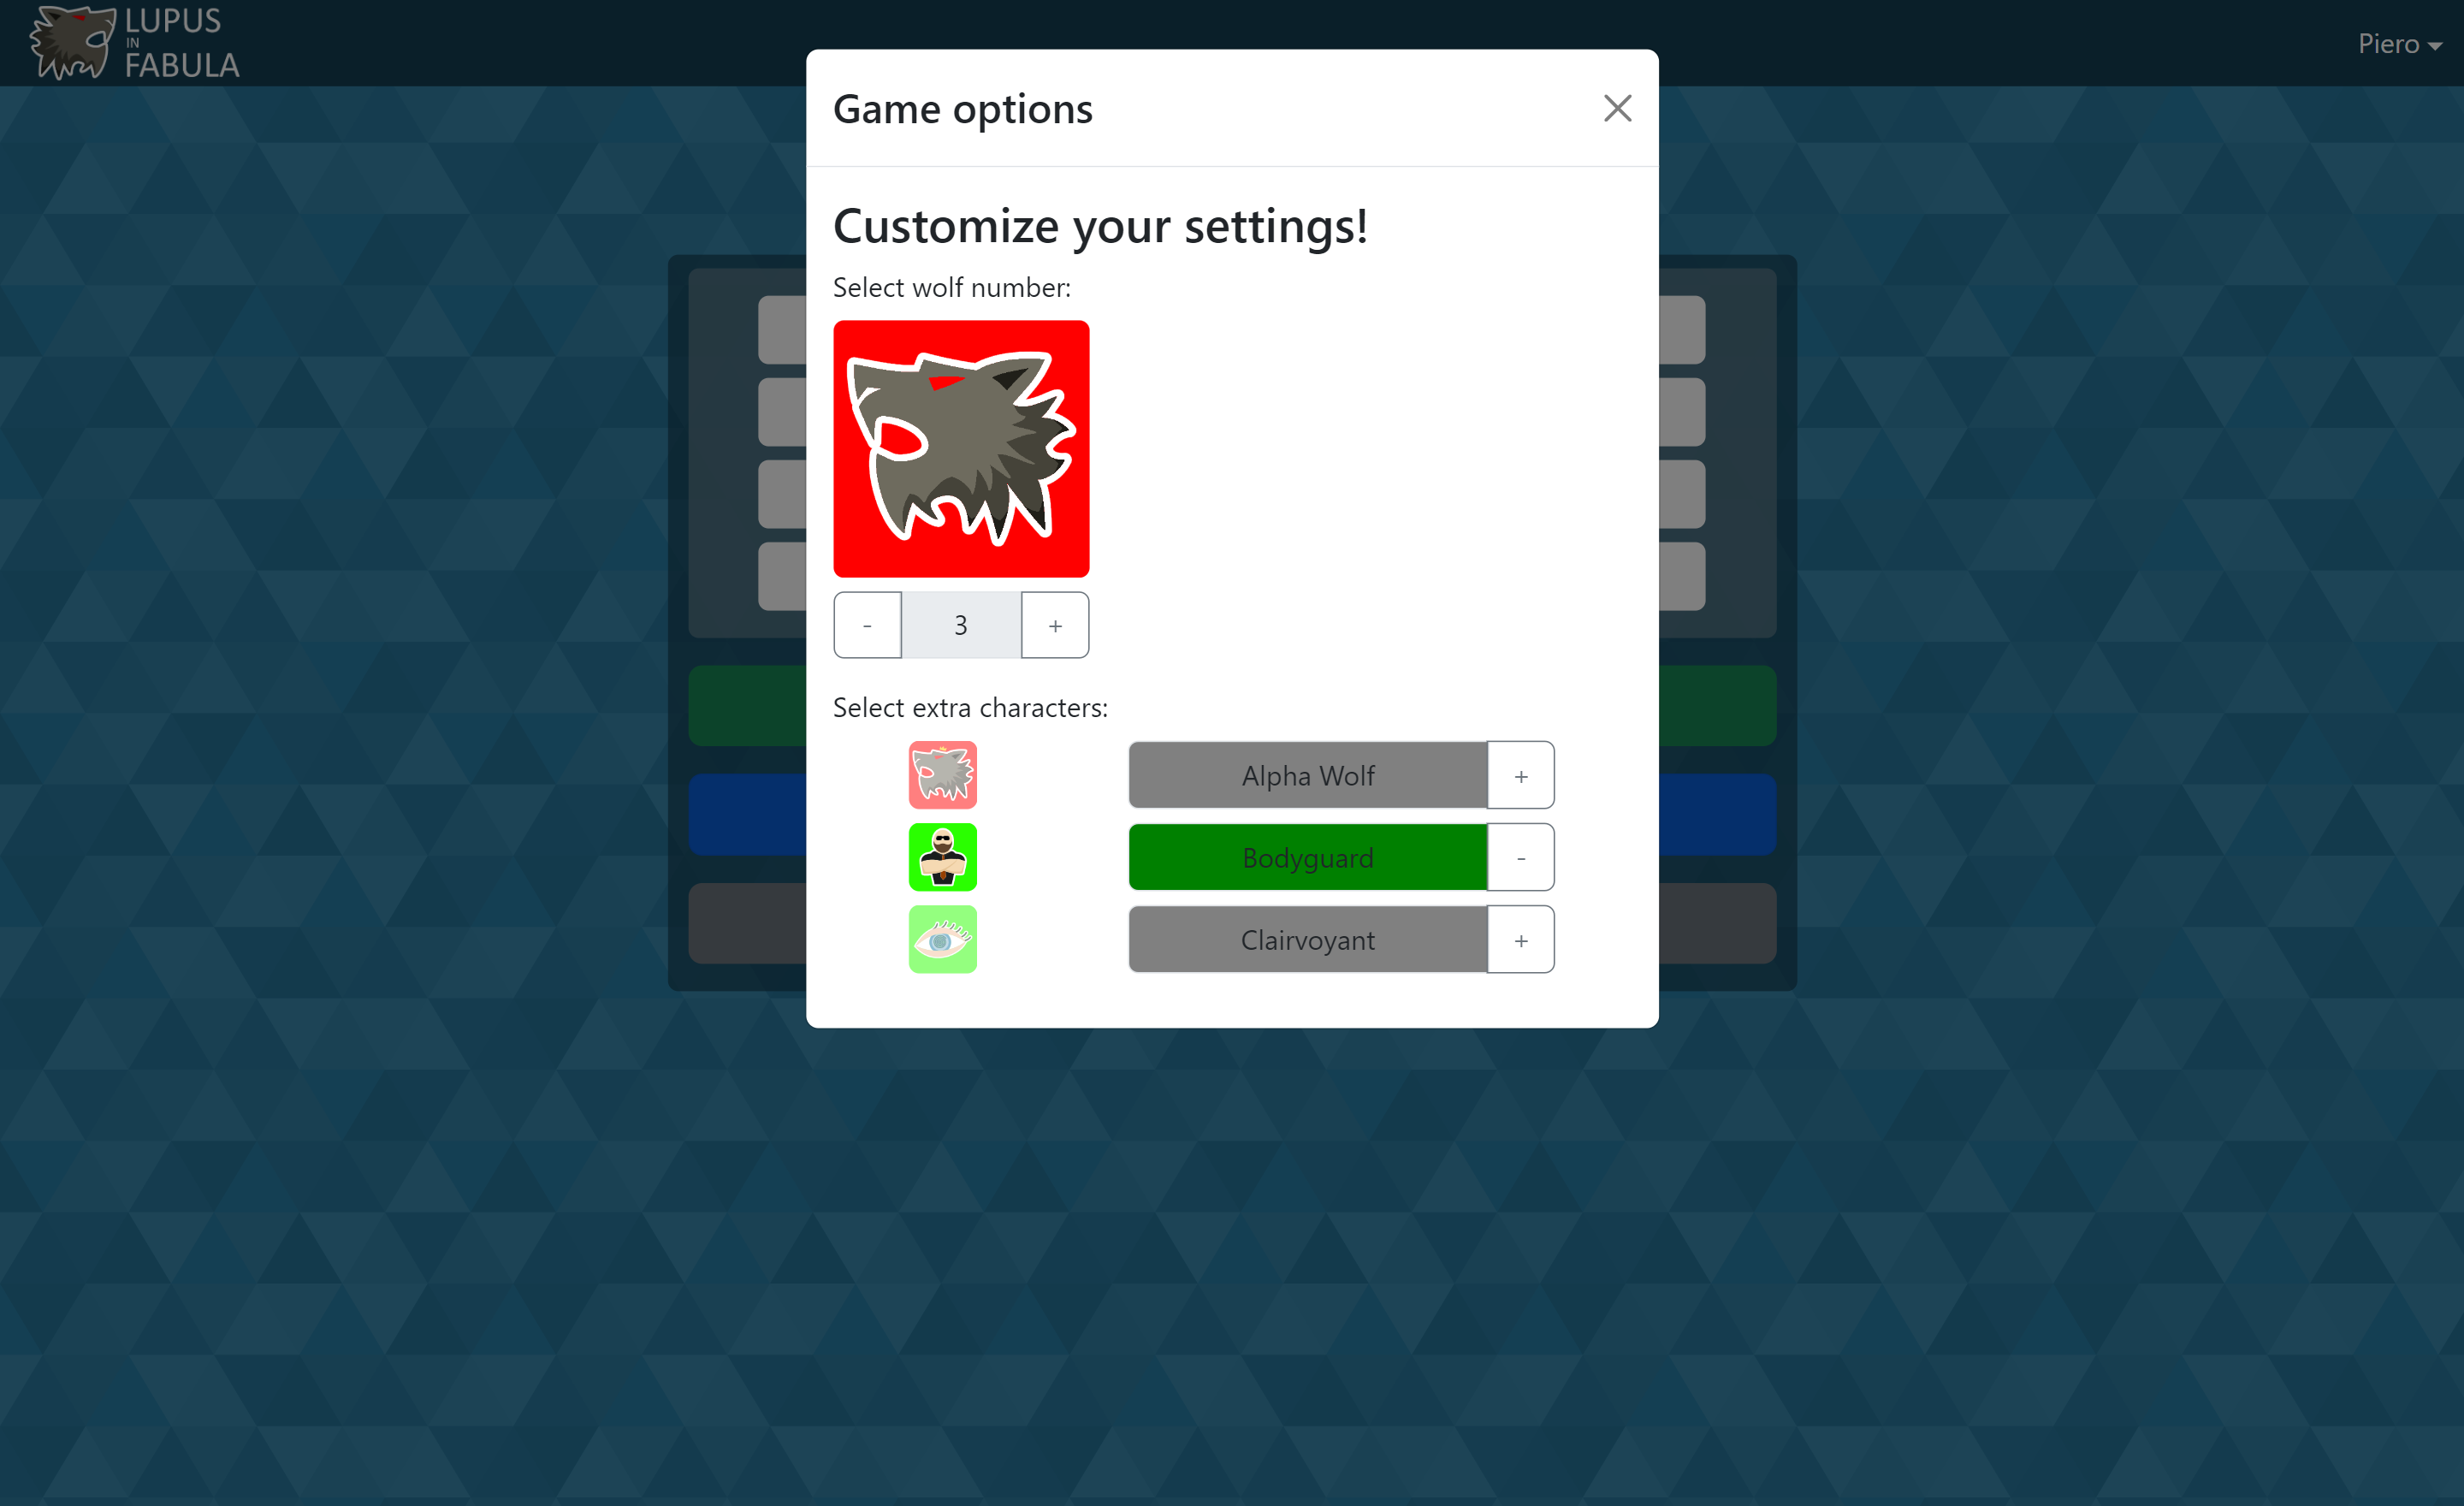
\includegraphics[width=0.95\textwidth]{img/screen/desktop/option_desktop.png}
    \end{minipage}
    \caption{Schermata delle opzioni}
    \label{fig:option_ui}
\end{figure}

Decisa la personalizzazione si può procedere ad avviare la partita, che per prima cosa mostrerà il ruolo assegnato in maniera casuale a ogni giocatore, come mostrato nella figura \ref{fig:card_ui}.


\begin{figure}[H]
    \centering
    \begin{minipage}{0.25\textwidth}
        \centering
        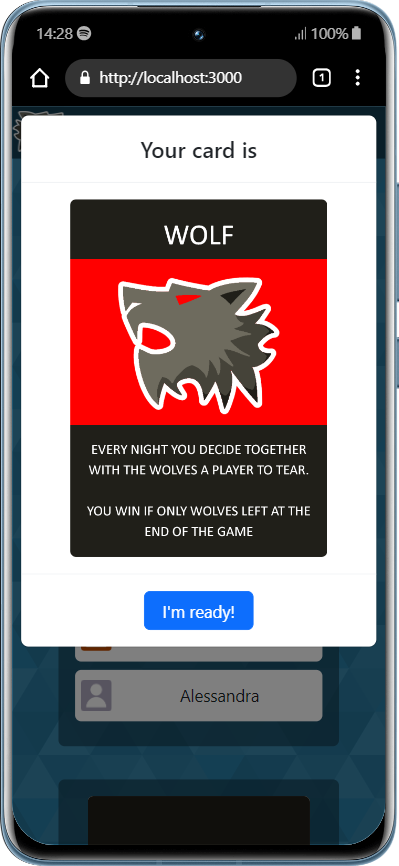
\includegraphics[width=0.95\textwidth]{img/screen/mobile/card_mobile.png}
    \end{minipage}\hfill
    \begin{minipage}{0.75\textwidth}
        \centering
        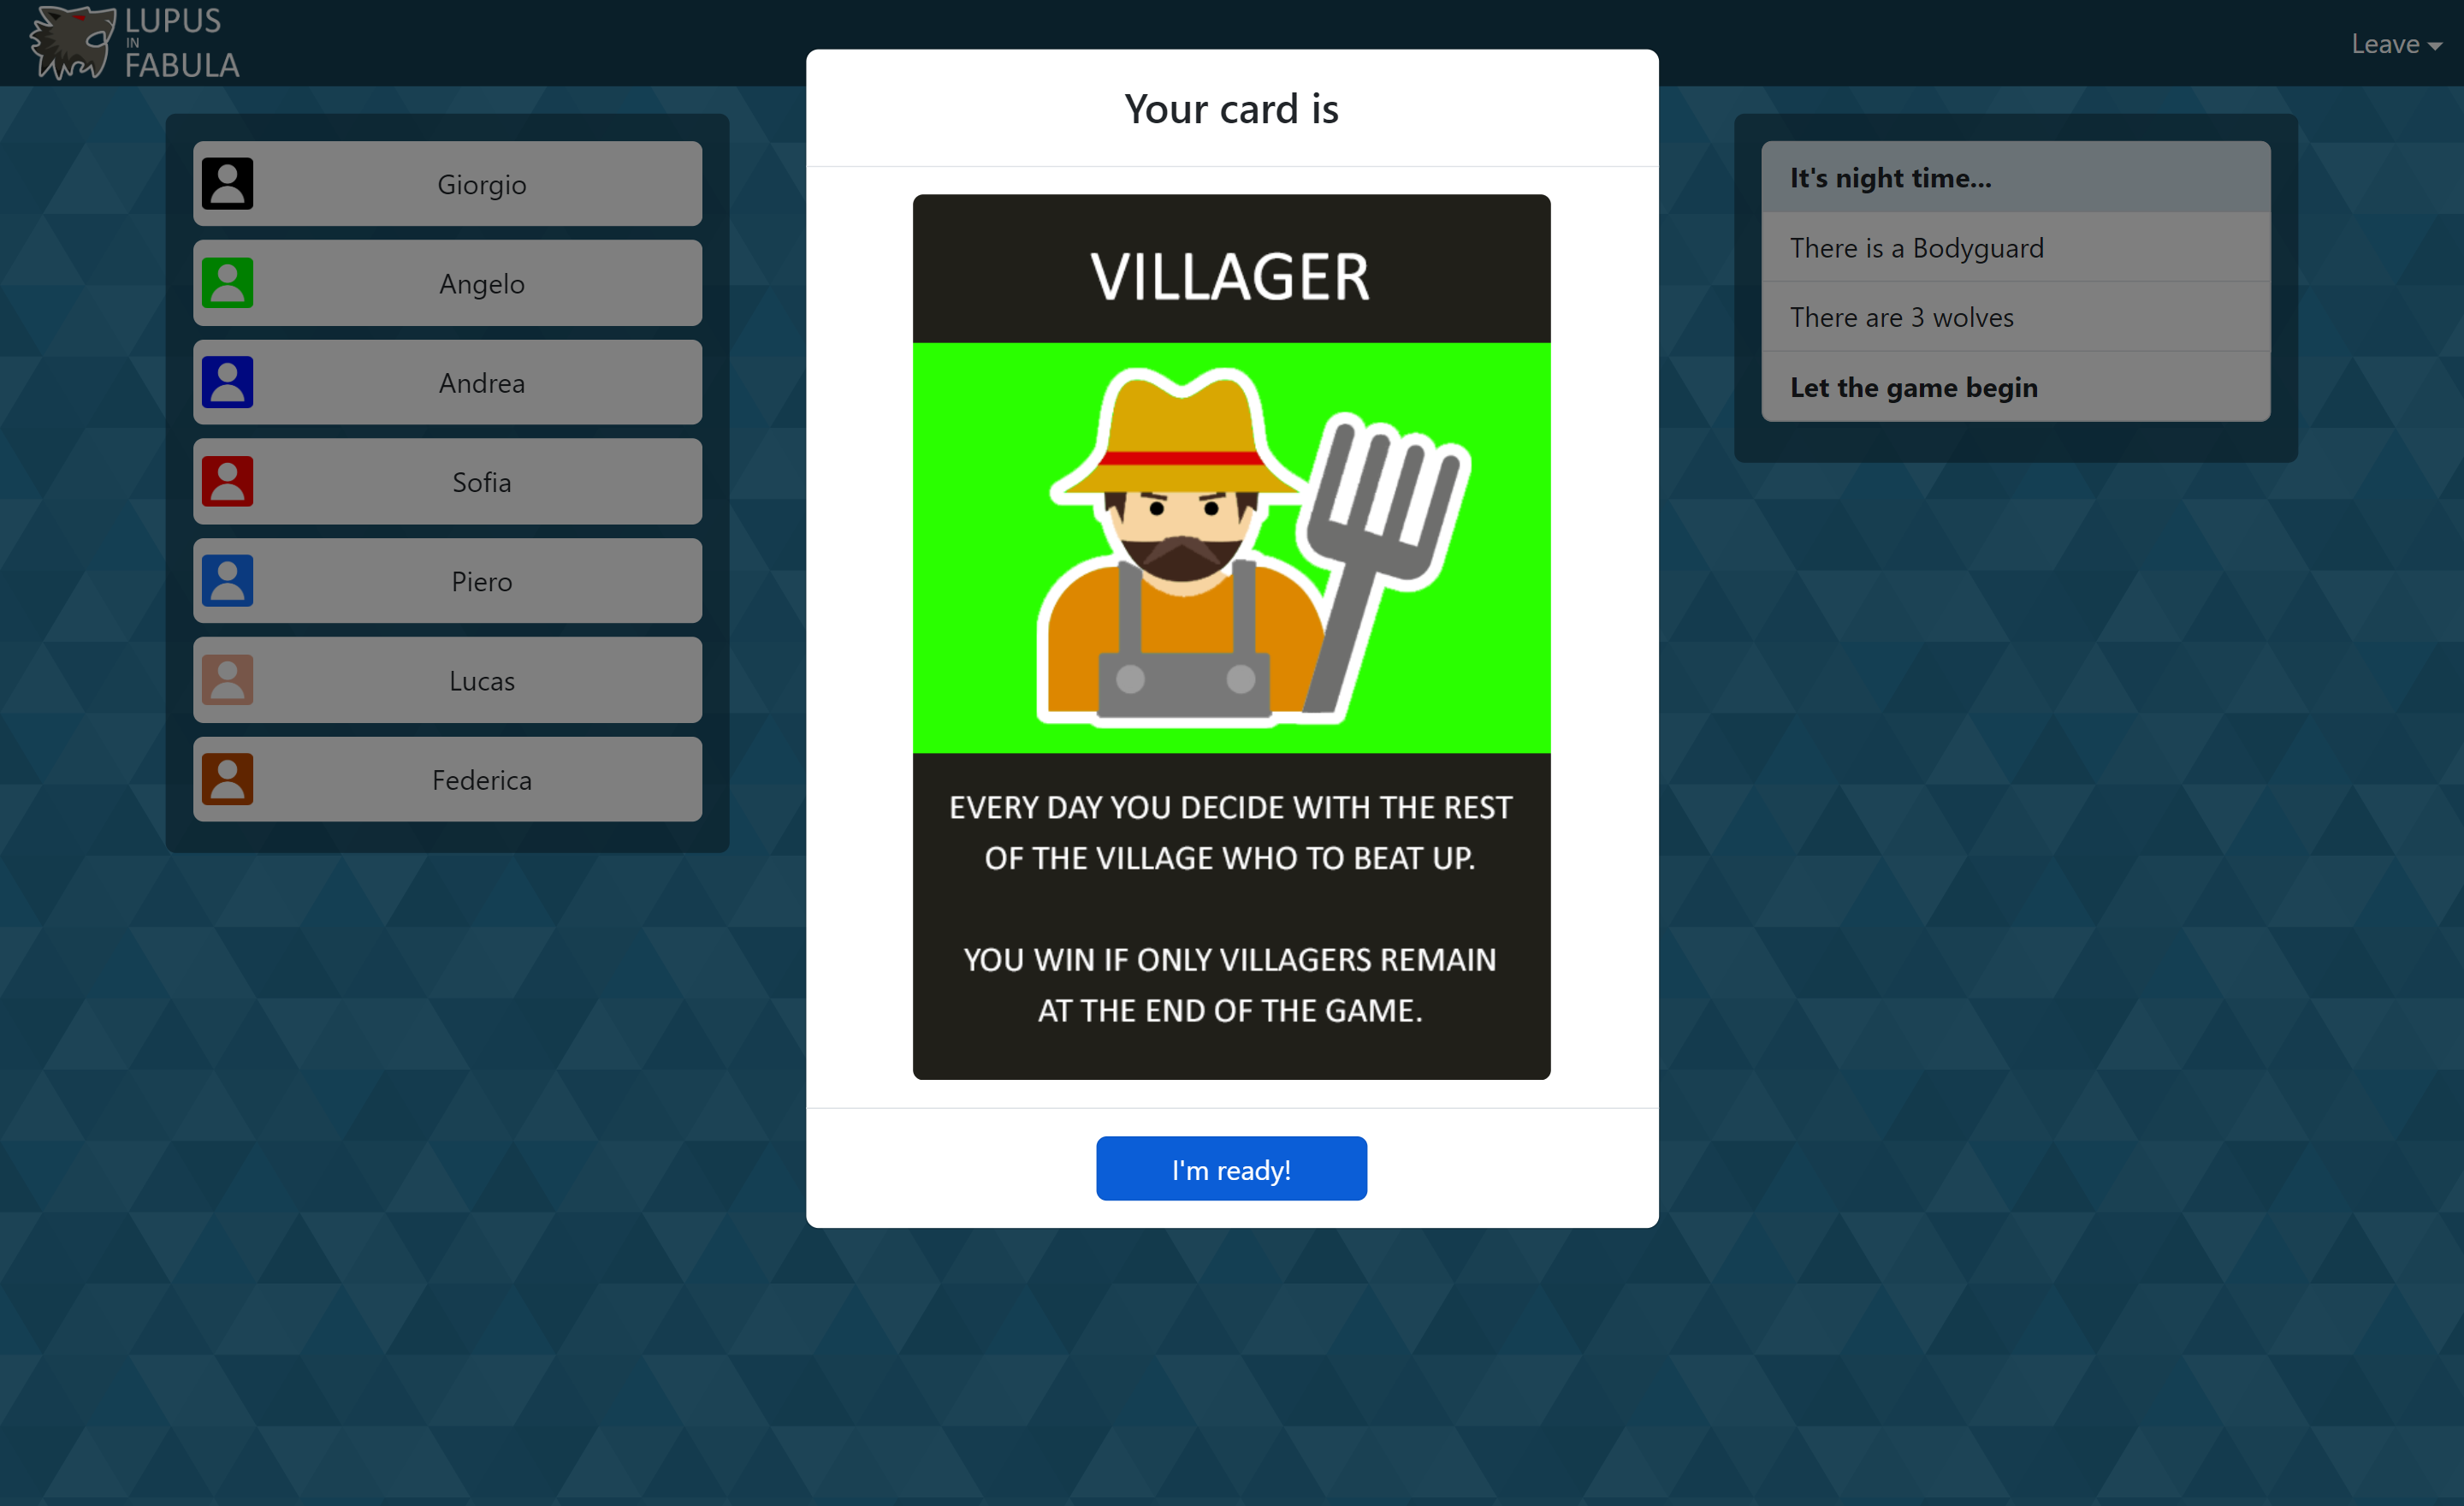
\includegraphics[width=0.95\textwidth]{img/screen/desktop/card_desktop.png}
    \end{minipage}
    \caption{Schermata di inizio partita}
    \label{fig:card_ui}
\end{figure}

Durante i turni di gioco ai partecipanti verrà richiesto di votare per portare a termine un'azione, uccidere, proteggere, svelare, o come nel caso riportato nella figura \ref{fig:accusation_ui}, accusare uno degli altri giocatori.

\begin{figure}[H]
    \centering
    \begin{minipage}{0.25\textwidth}
        \centering
        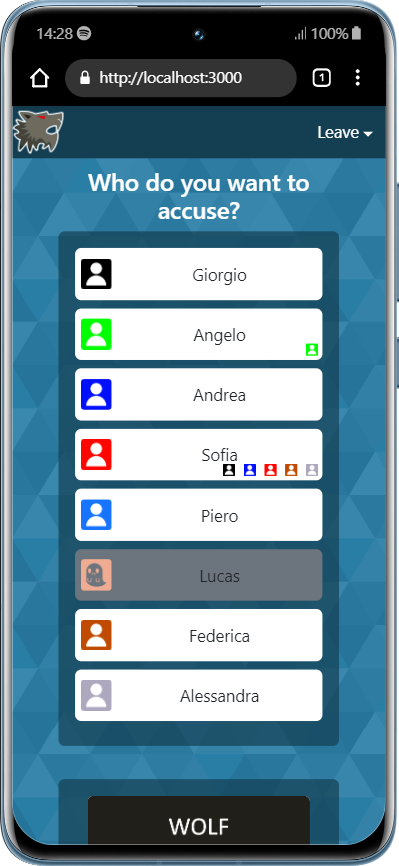
\includegraphics[width=0.95\textwidth]{img/screen/mobile/accusation_mobile.png}
    \end{minipage}\hfill
    \begin{minipage}{0.75\textwidth}
        \centering
        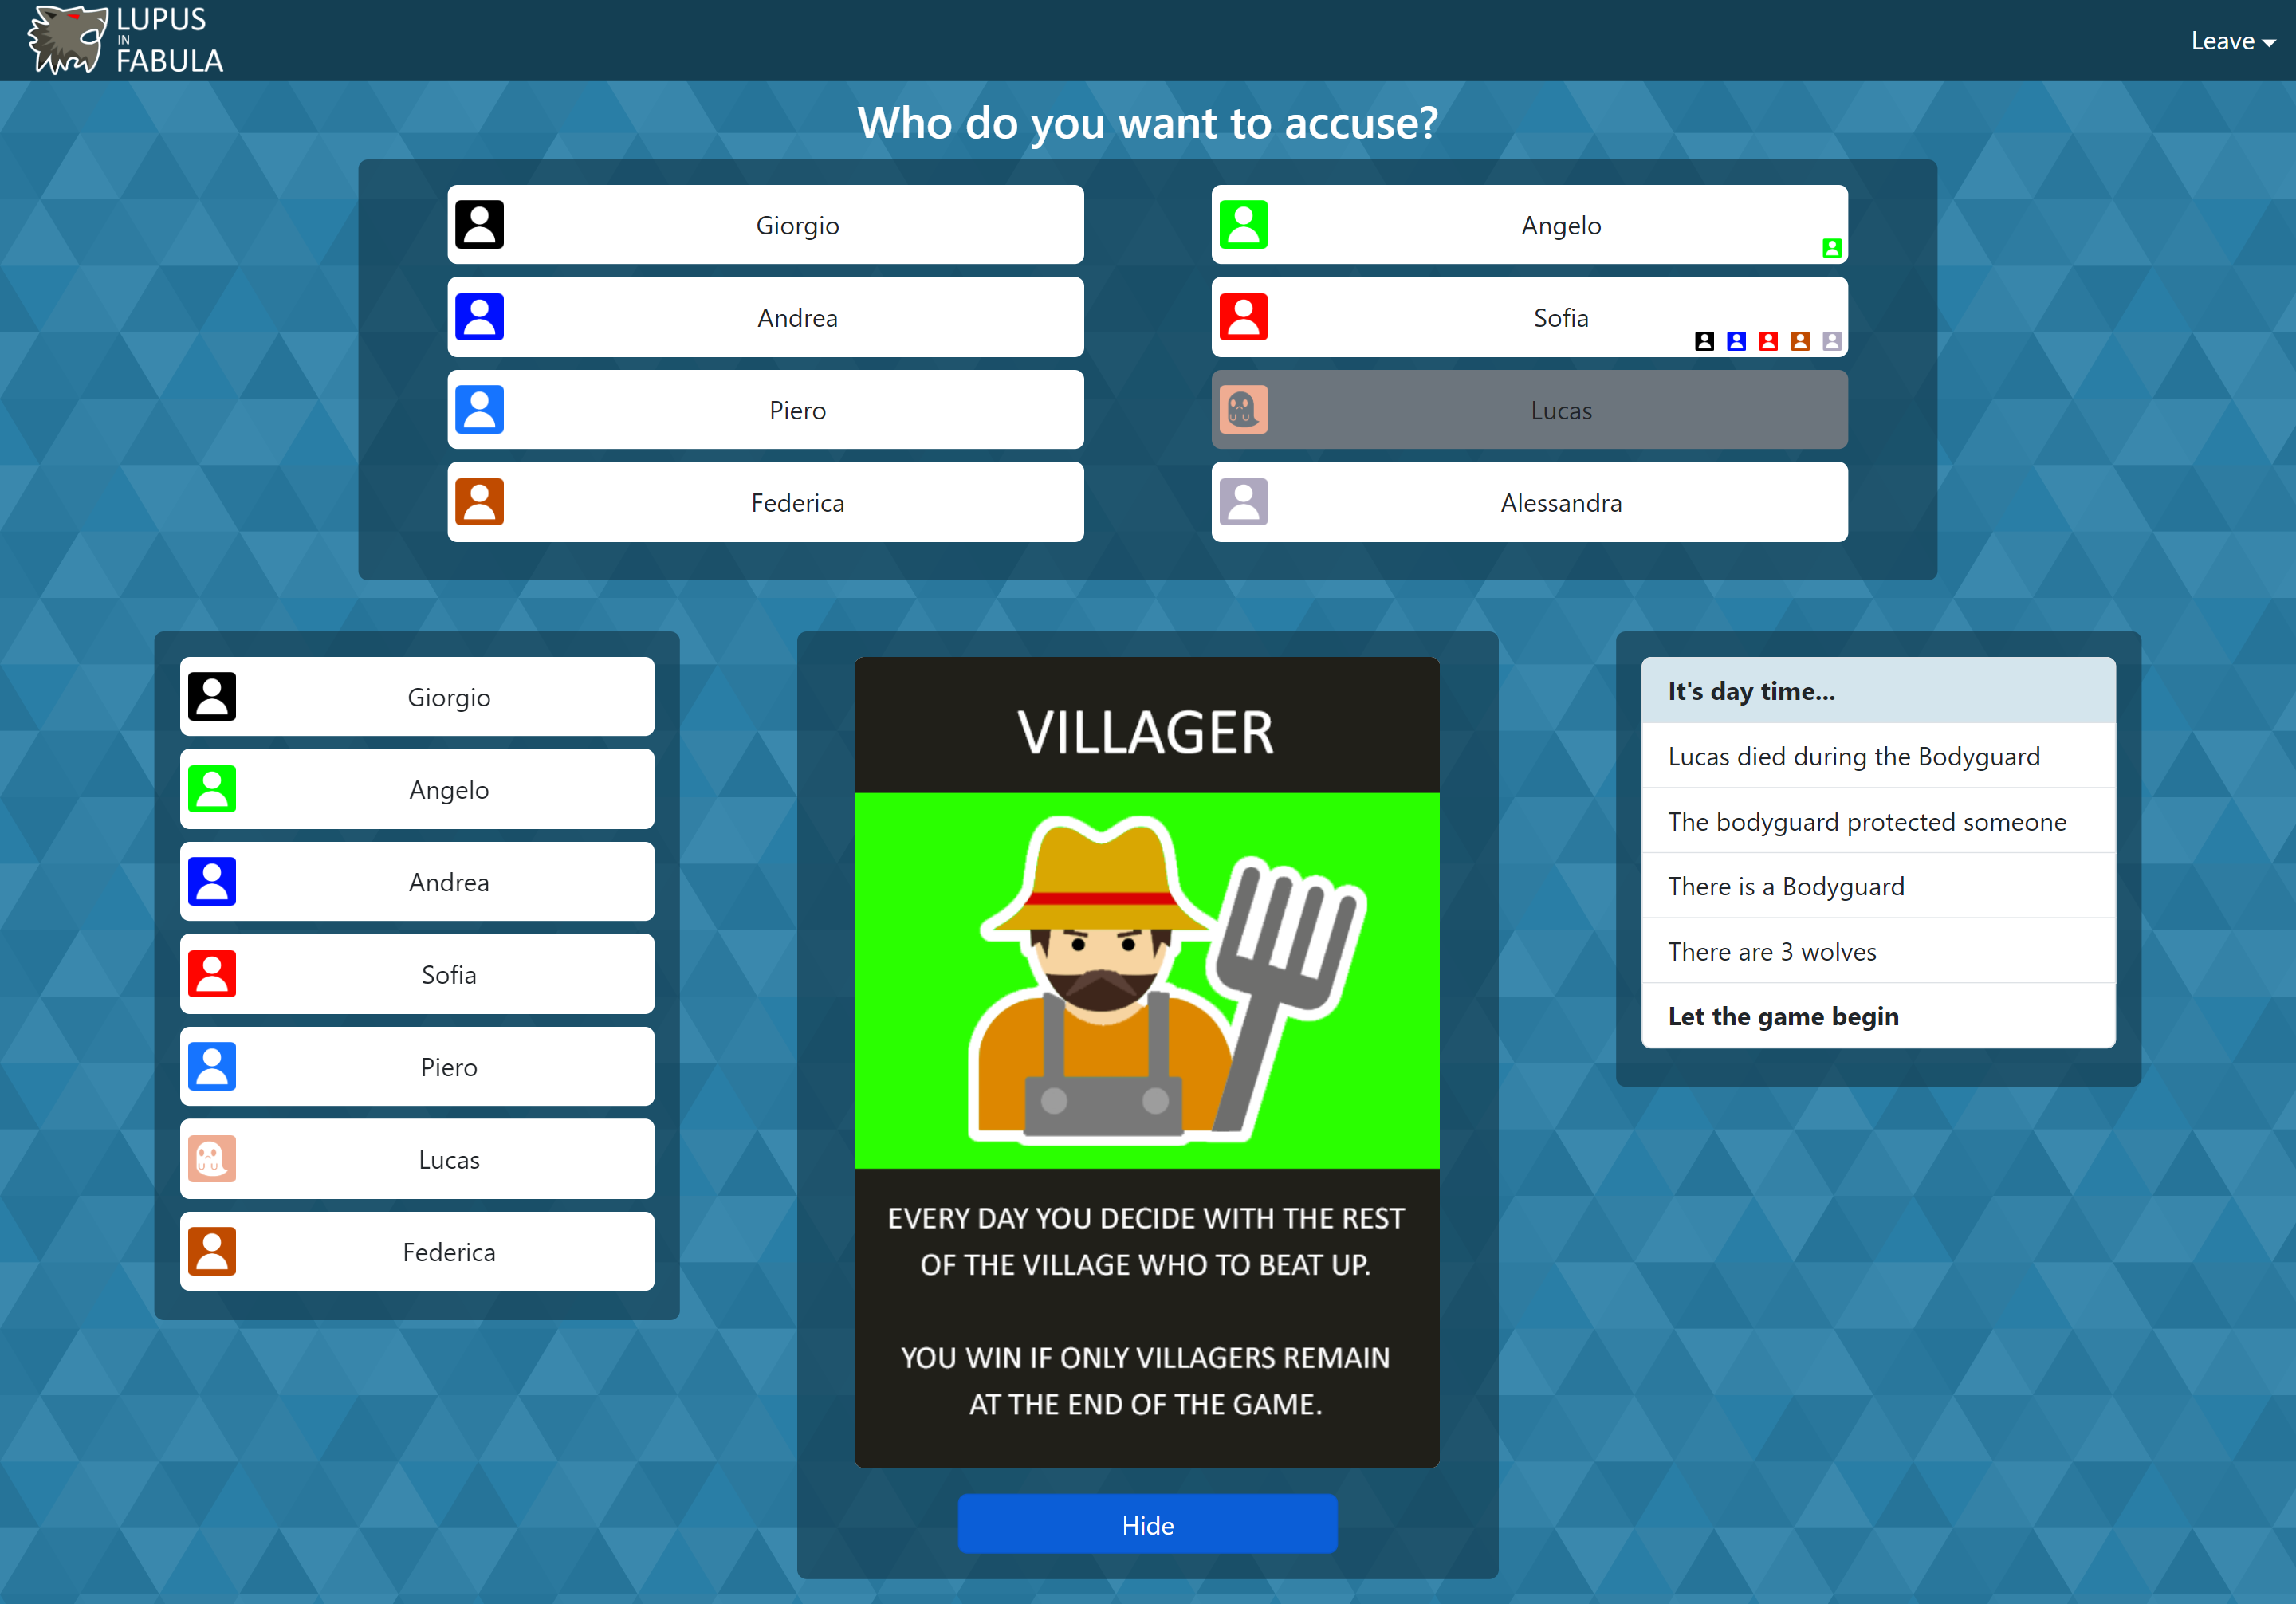
\includegraphics[width=0.95\textwidth]{img/screen/desktop/accusation_desktop.png}
    \end{minipage}
    \caption{Schermata di turno di accusa}
    \label{fig:accusation_ui}
\end{figure}

Nella figura \ref{fig:dead_ui} si può vedere la schermata che viene mostrata ai giocatori che muoiono durante la partita. In quest'ultima sarà possibile continuare a seguire gli avvenimenti della partita, ricoprendo un ruolo onnisciente per quanto riguarda le carte distribuite agli altri giocatori.

\begin{figure}[H]
    \centering
    \begin{minipage}{0.25\textwidth}
        \centering
        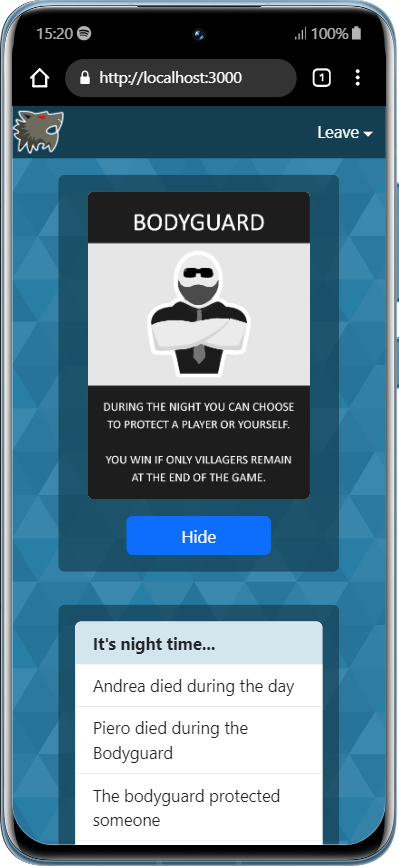
\includegraphics[width=0.95\textwidth]{img/screen/mobile/dead_mobile.png}
    \end{minipage}\hfill
    \begin{minipage}{0.75\textwidth}
        \centering
        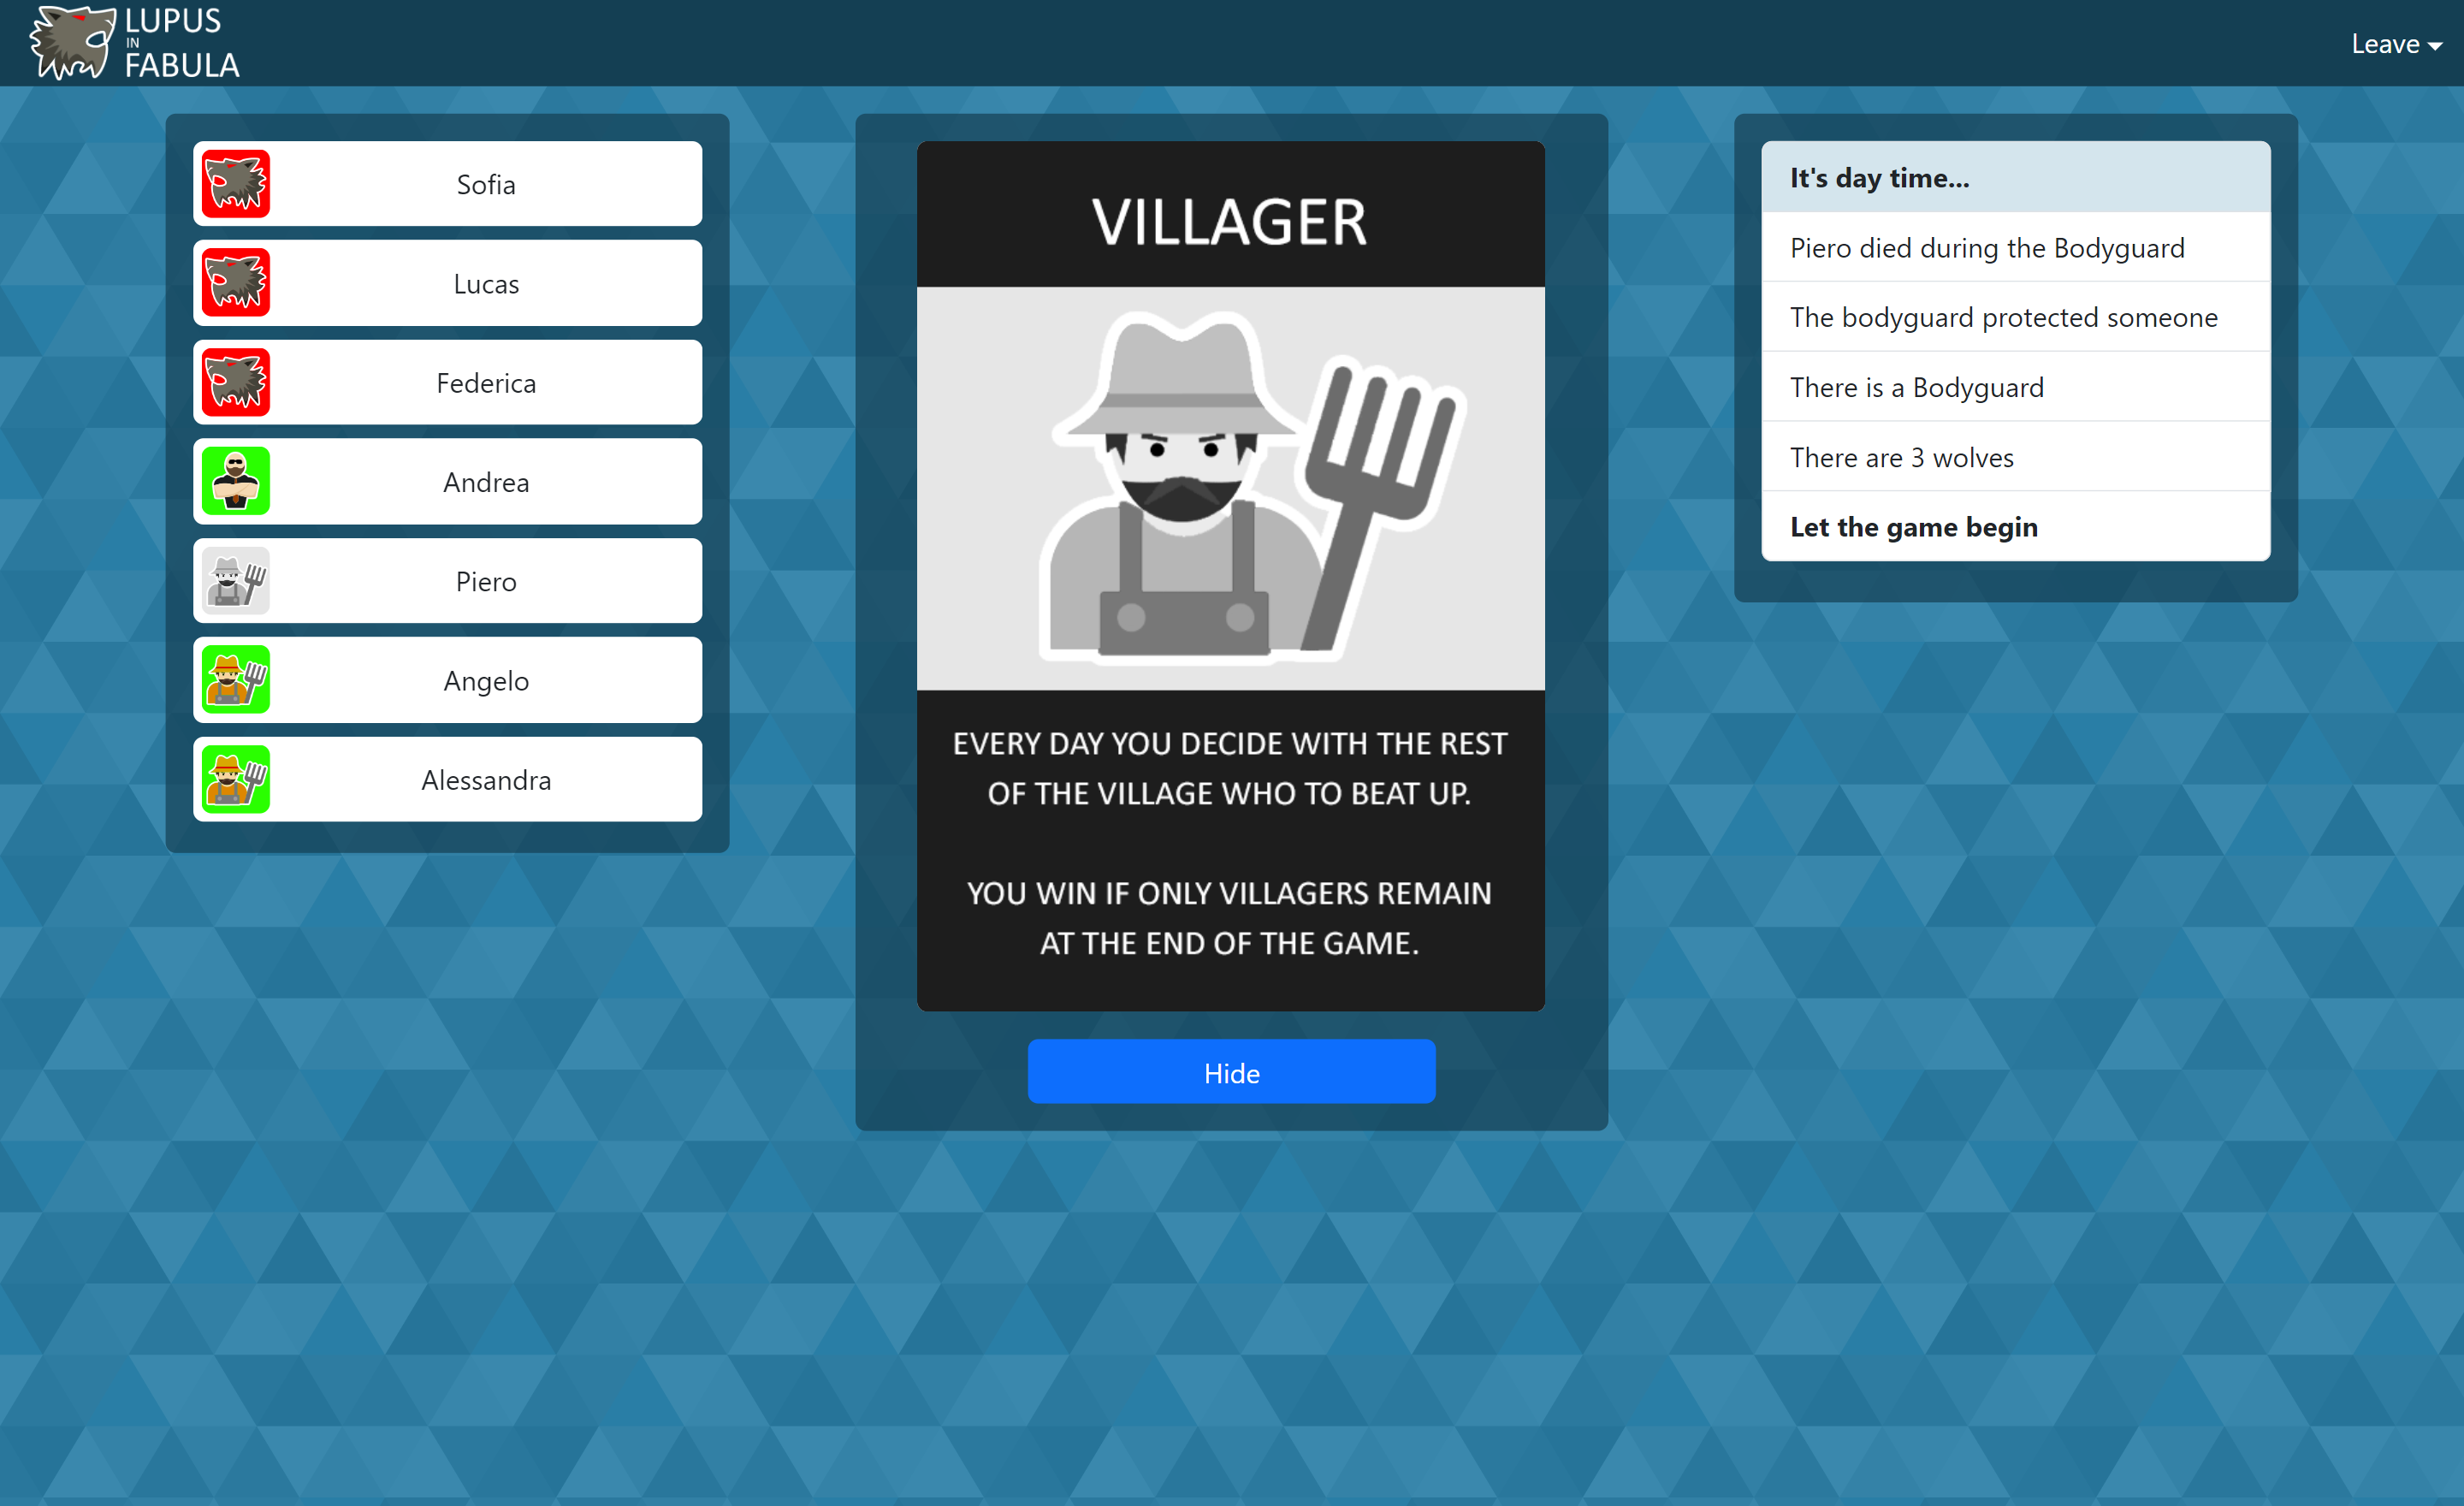
\includegraphics[width=0.95\textwidth]{img/screen/desktop/dead_desktop.png}
    \end{minipage}
    \caption{Schermata del giocatore morto}
    \label{fig:dead_ui}
\end{figure}

Al termine della partita verrà infine mostrata una schermata riassuntiva delle due squadre, indicando come visibile nella figura \ref{fig:won_ui} quale delle due abbia vinto e quali membri siano stati uccisi durante il susseguirsi delle fasi. Da qui sarà possibile salvare l'esito della partita sul database oppure procedere direttamente a iniziarne una nuova.

\begin{figure}[H]
    \centering
    \begin{minipage}{0.25\textwidth}
        \centering
        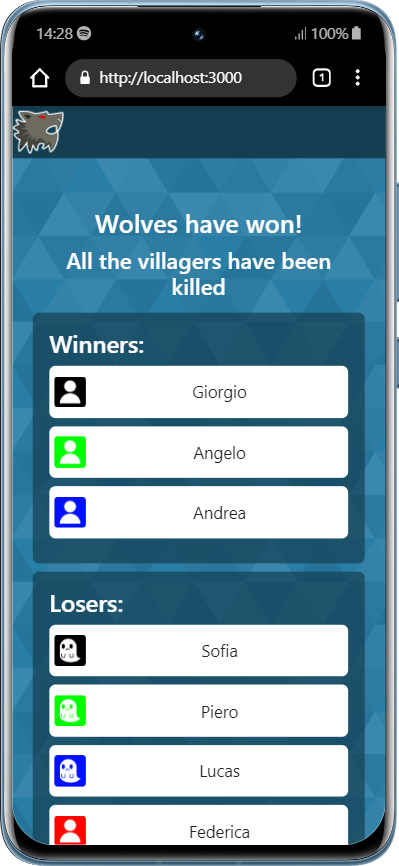
\includegraphics[width=0.95\textwidth]{img/screen/mobile/won_mobile.png}
    \end{minipage}\hfill
    \begin{minipage}{0.75\textwidth}
        \centering
        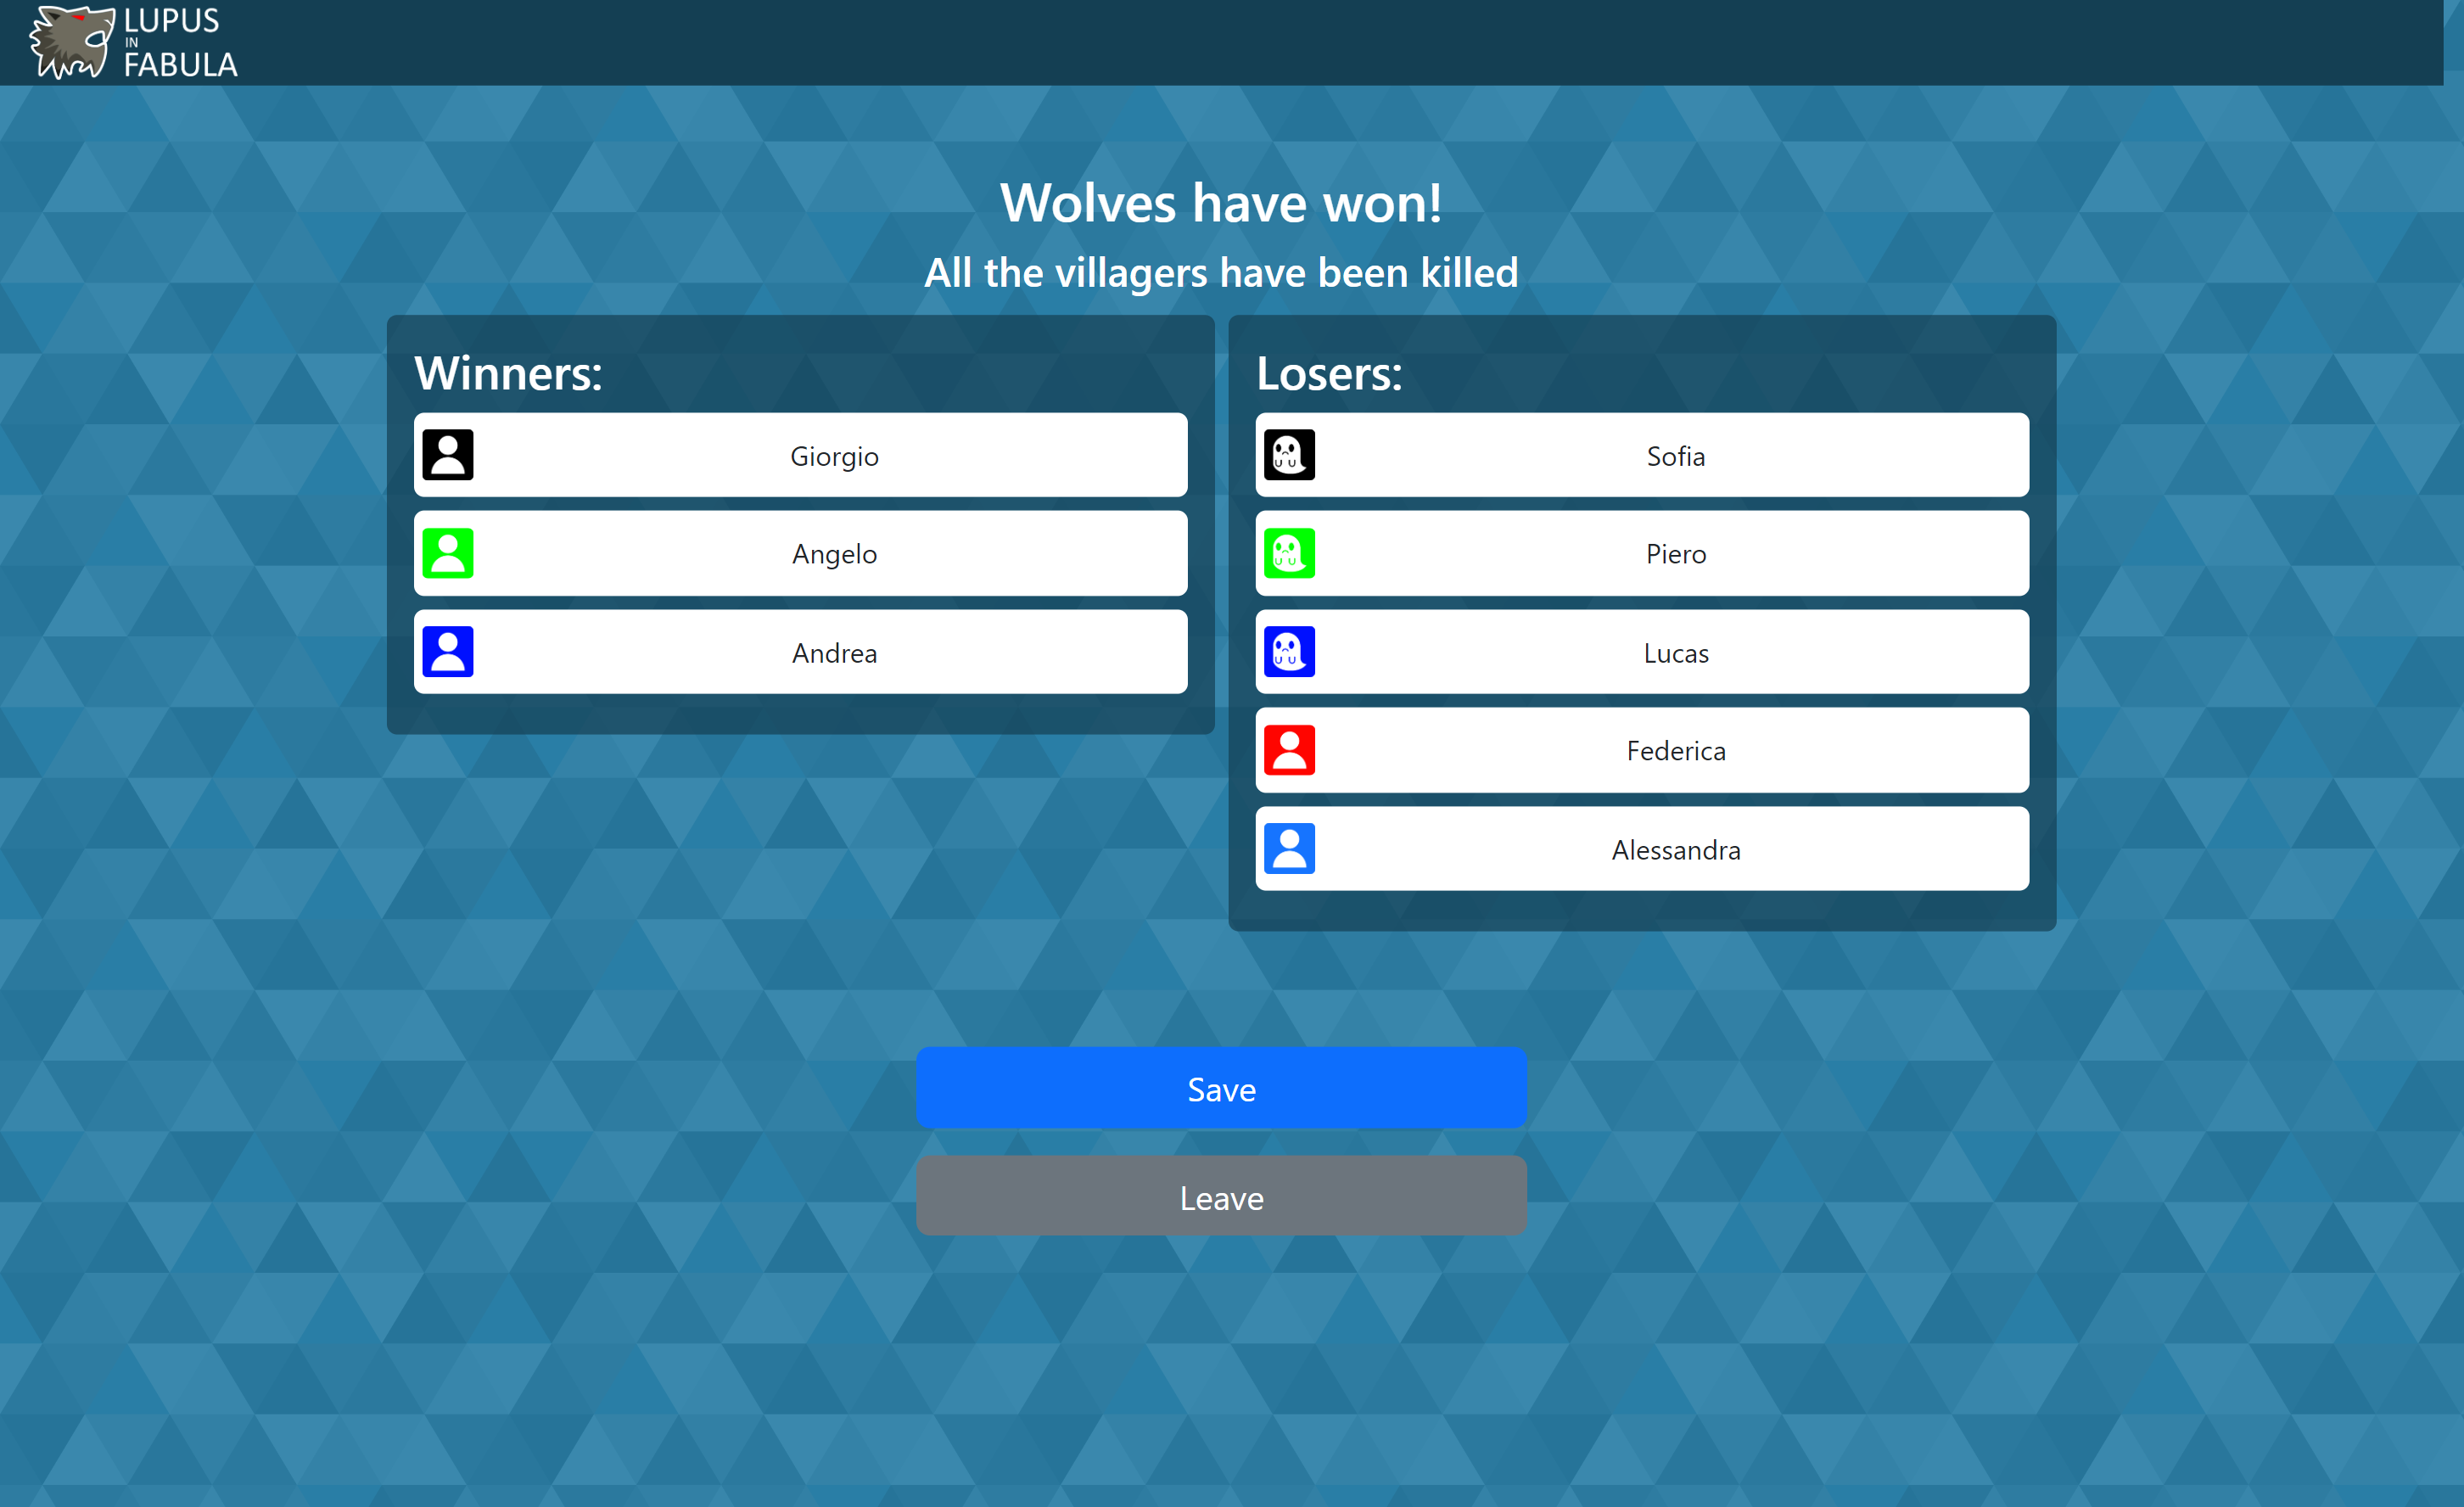
\includegraphics[width=0.95\textwidth]{img/screen/desktop/won_desktop.png}
    \end{minipage}
    \caption{Schermata di fine partita}
    \label{fig:won_ui}
\end{figure}

Come per la schermata di selezione della lingua, una volta effettuato il login sarà possibile per l'utente, sempre utilizzando il menù a tendina in alto a destra, visualizzare le proprie statistiche di gioco.

\begin{figure}[H]
    \centering
    \begin{minipage}{0.25\textwidth}
        \centering
        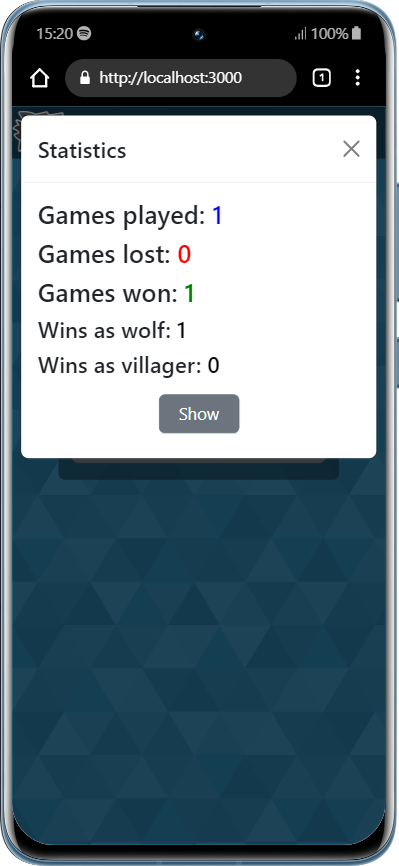
\includegraphics[width=0.95\textwidth]{img/screen/mobile/stats_mobile.png}
    \end{minipage}\hfill
    \begin{minipage}{0.75\textwidth}
        \centering
        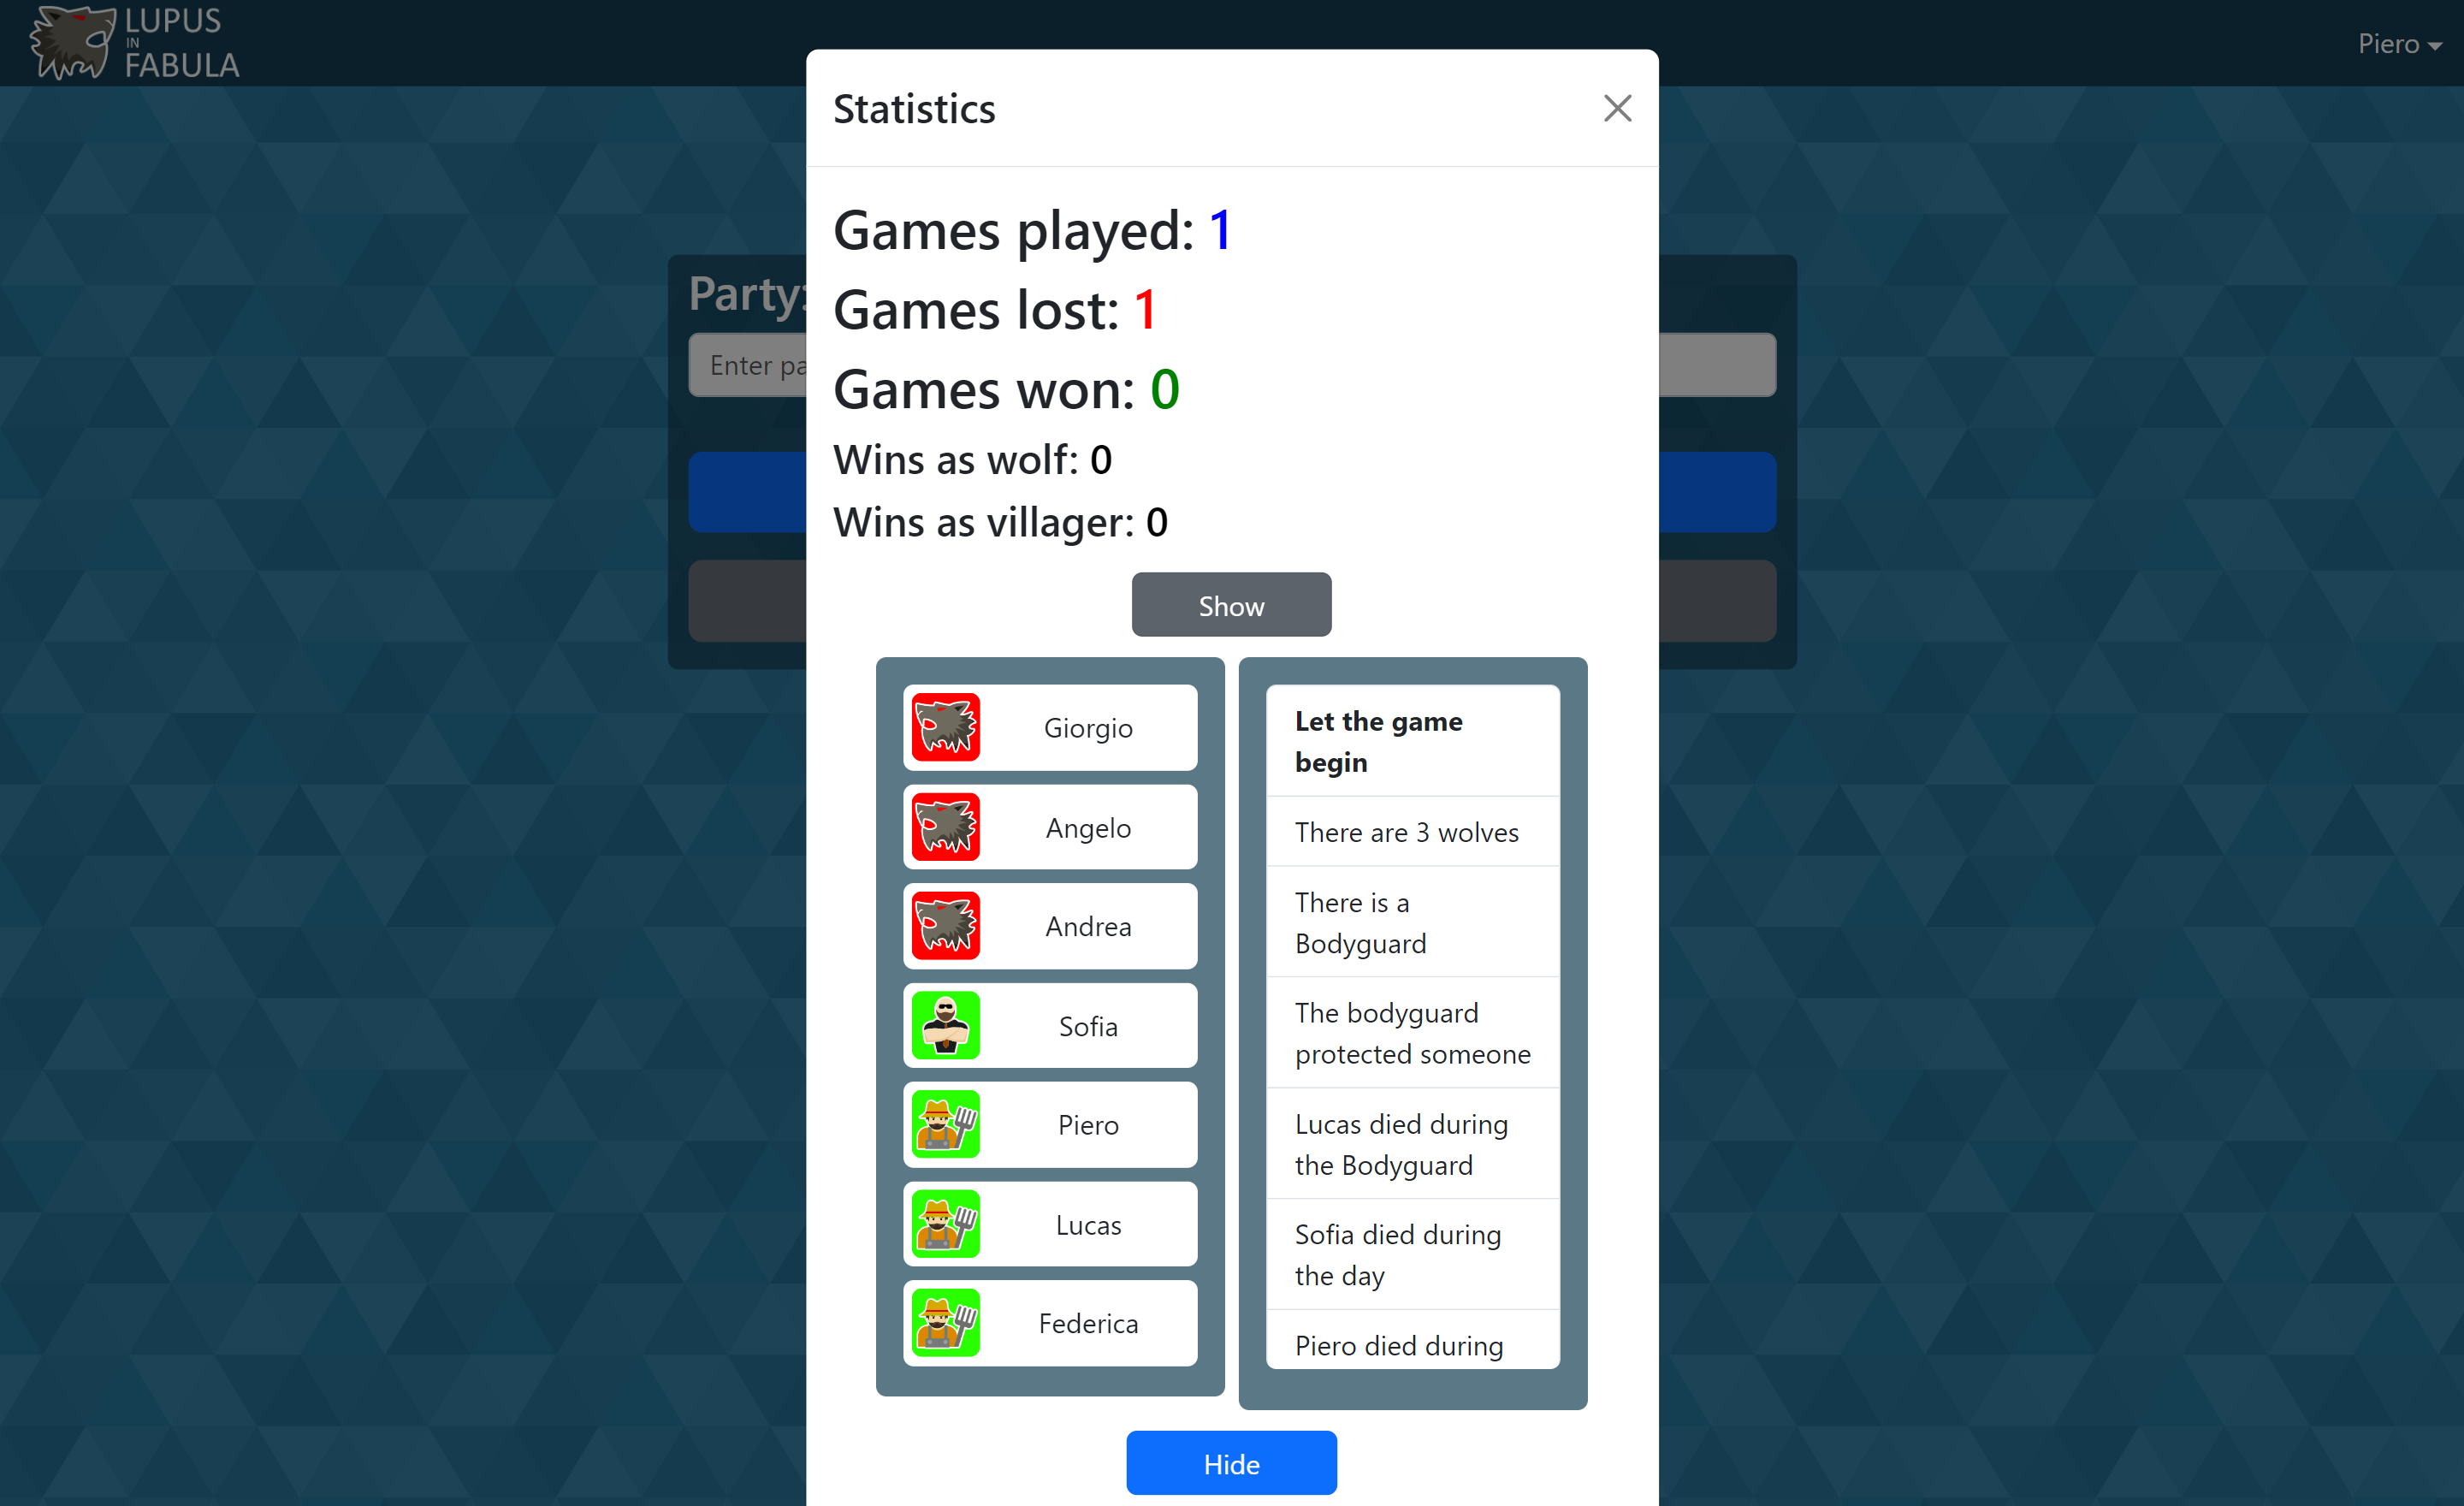
\includegraphics[width=0.95\textwidth]{img/screen/desktop/stats_desktop.png}
    \end{minipage}
    \caption{Schermata delle statistiche del giocatore}
    \label{fig:stats_ui}
\end{figure}

Nel caso un utente infine provasse a navigare al di fuori dei percorsi definiti all'interno del sistema l'interfaccia che gli verrà presentata sarà quella visibile nella figura \ref{fig:404_ui}, attraverso la quale sarà possibile ritornare alla pagina iniziale.

\begin{figure}[H]
    \centering
    \begin{minipage}{0.25\textwidth}
        \centering
        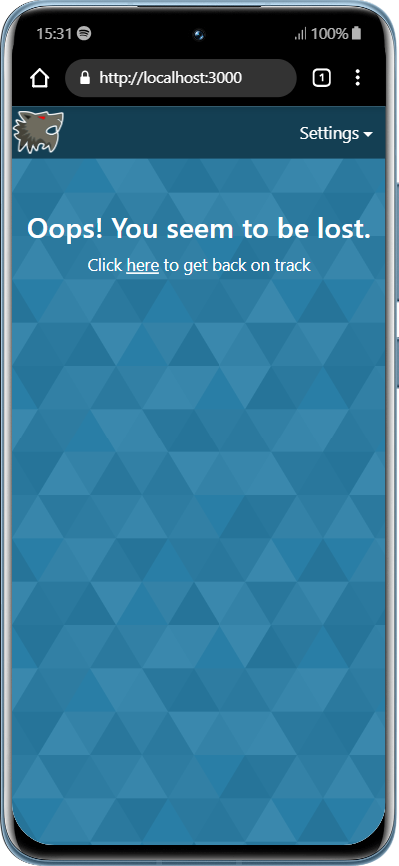
\includegraphics[width=0.95\textwidth]{img/screen/mobile/404_mobile.png}
    \end{minipage}\hfill
    \begin{minipage}{0.75\textwidth}
        \centering
        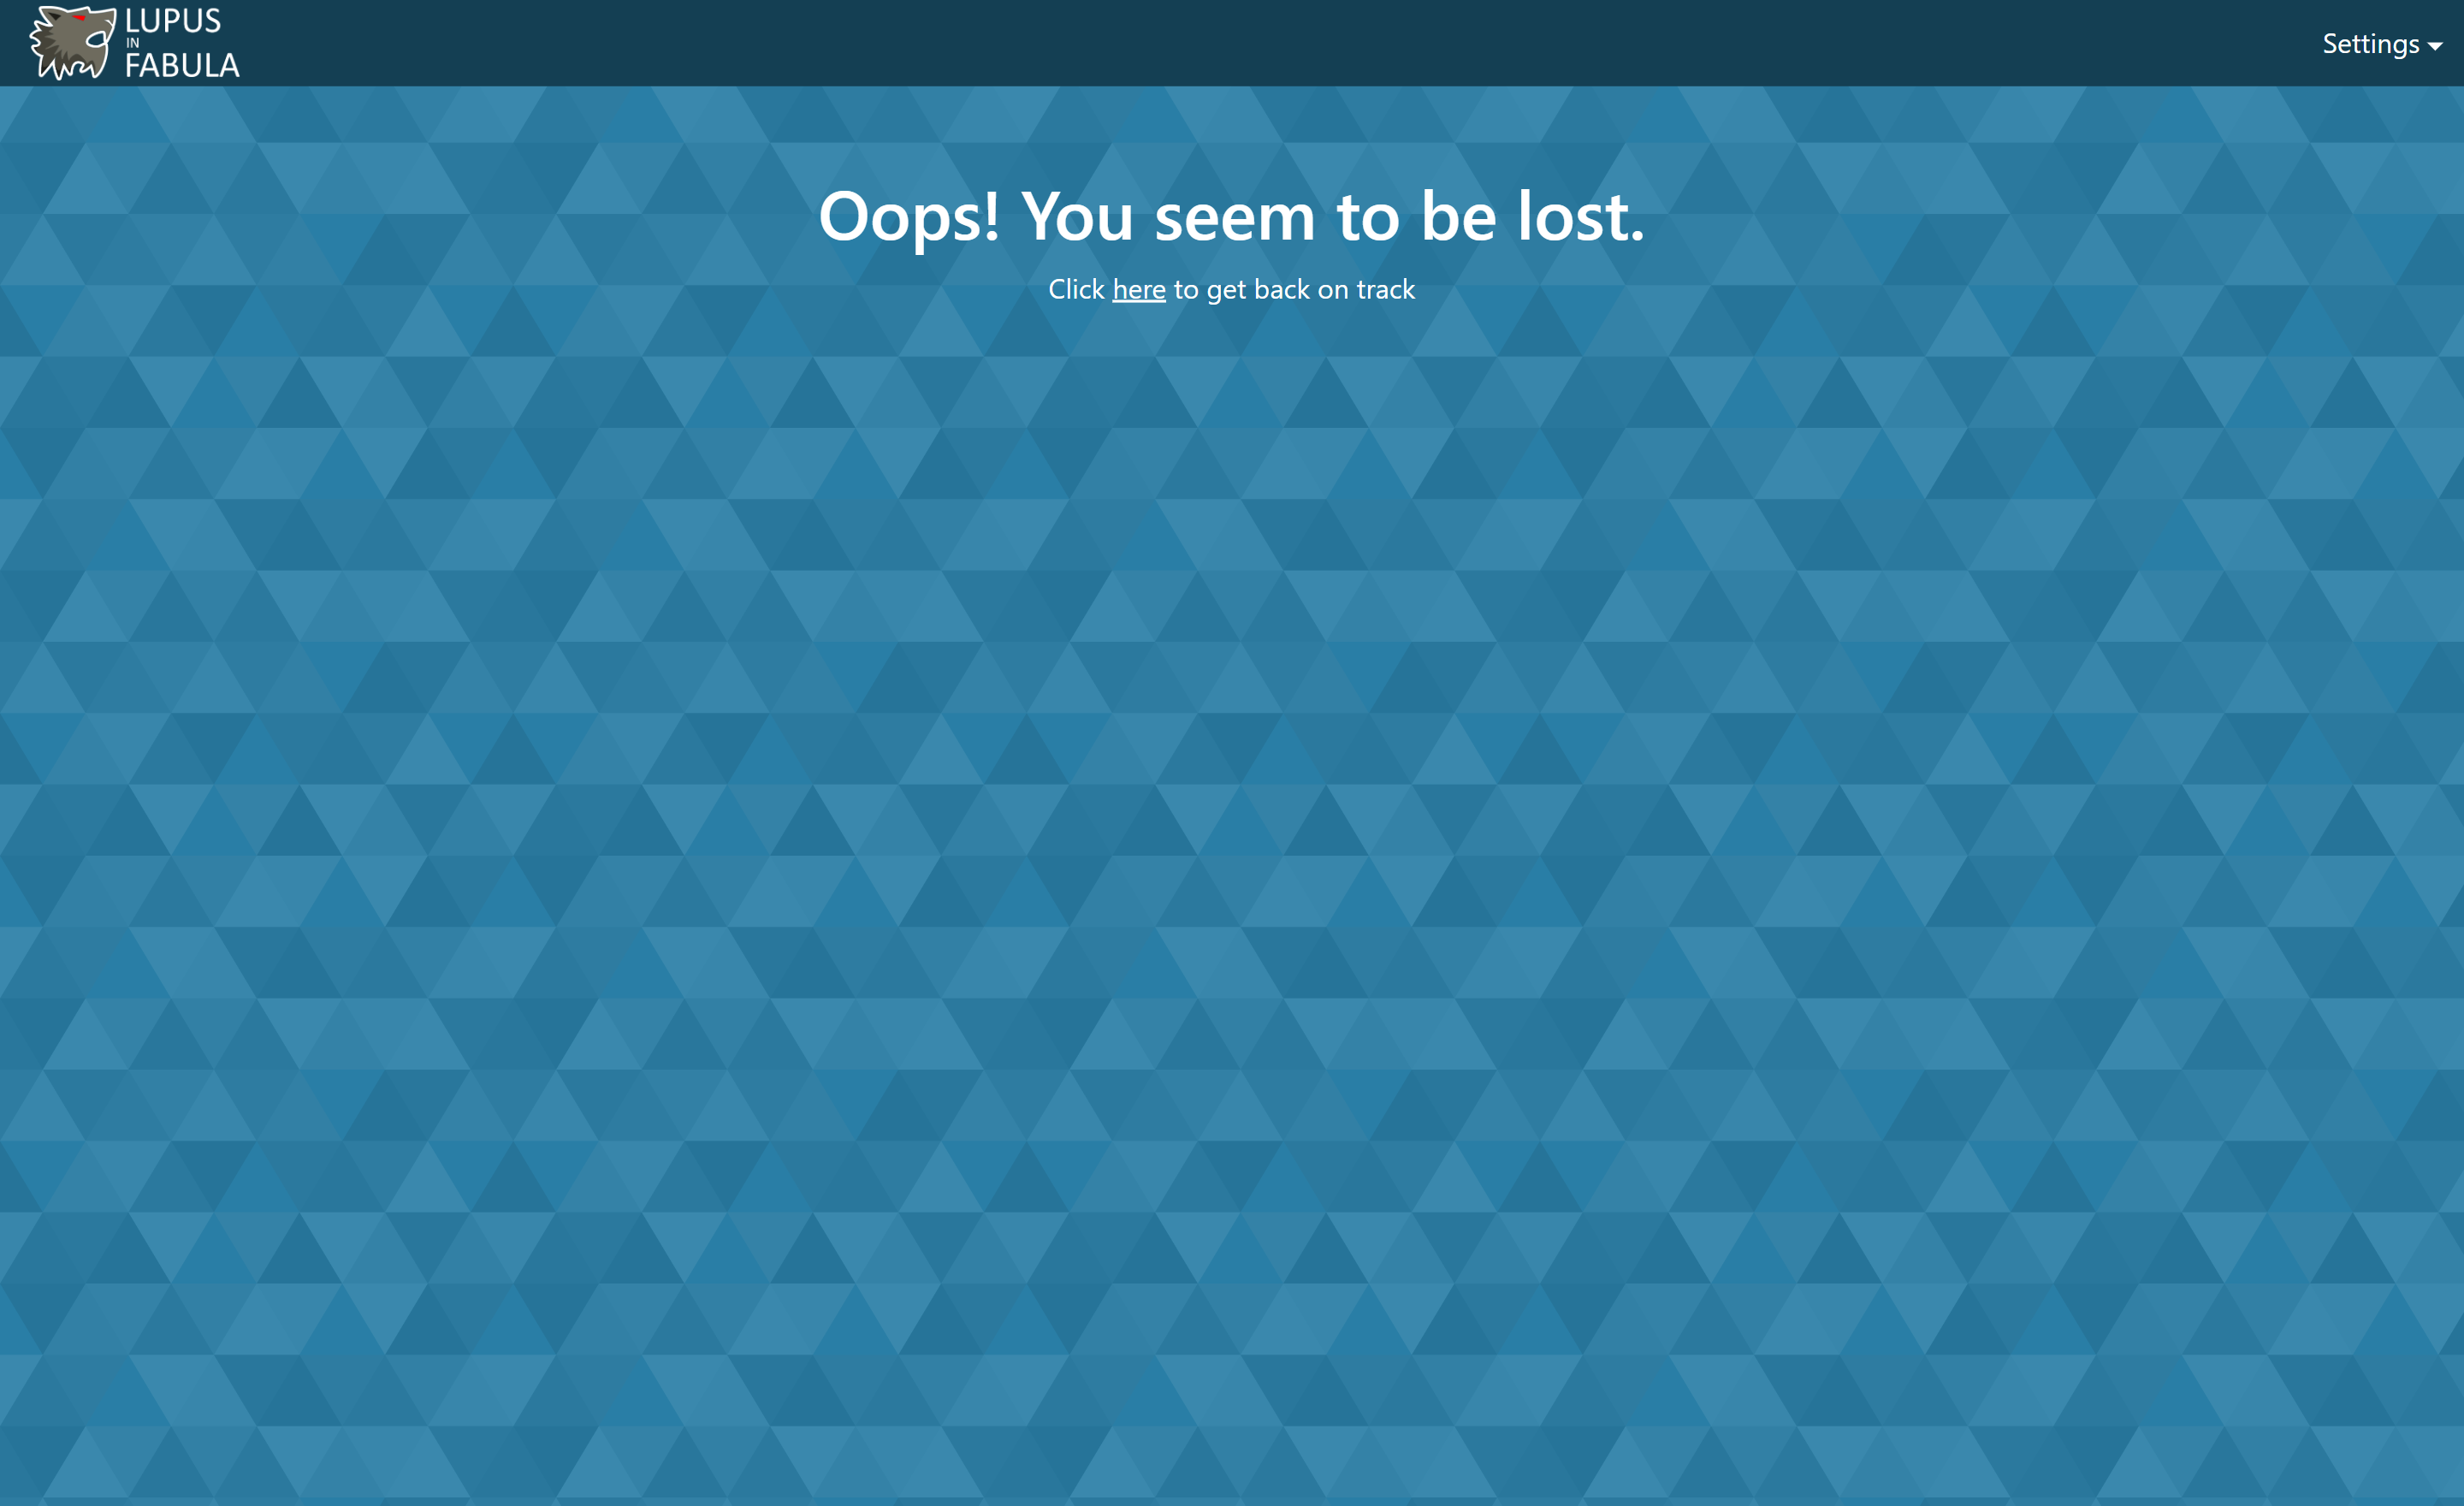
\includegraphics[width=0.95\textwidth]{img/screen/desktop/404_desktop.png}
    \end{minipage}
    \caption{Schermata 404 indirizzo non trovato}
    \label{fig:404_ui}
\end{figure}
